\documentclass{article}
\usepackage[utf8]{inputenc}
\usepackage{xcolor}
\usepackage{geometry}
\usepackage{graphicx}
\usepackage{amsmath}
\usepackage[spanish]{babel}

\newcommand{\set}[1]{\{#1\}}

\title{
  Introducci\'on al procesamiento digital de im\'agenes \\
  {\bf TP 3: Compresi\'on}
}
\author{
  Pablo Barenbaum \\
  Juli\'an Bayardo
}
\date{}

\newcommand{\TODO}[1]{\textcolor{red}{TODO: #1}}

\begin{document}
\maketitle
\tableofcontents

\section{Introducción}

Este TP consiste en implementar una variante simplificada del método
de compresión JPEG para imágenes digitales.

El método JPEG proviene de un estándar especificado por el comité homónimo,
que data de fines de la década de 1980.
La variante simplificada que se implementa en este trabajo
dista mucho de la complejidad del estándar oficial.
Lo que se implementa es un prototipo minimal,
destinado a entender y poner a prueba sus mecanismos.

Una característica central del método de compresión JPEG es que es {\em lossy},
es decir, con pérdida de información,
lo que resulta en altas tasas de compresión,
con el costo aparejado de reducir la calidad de la imagen.
El componente central del método es la
transformada discreta del coseno (DCT), que representa la imagen
como una matriz de coeficientes en una base de funciones periódicas
(cosenos).
A continuación, los valores de estos coeficientes se truncan:
esta es la única etapa {\em lossy} del método.
Esta transformación es la que permite obtener altas tasas de compresión,
aplicando posteriormente otros métodos de compresión conocidos
(sin pérdida de información) tales como {\em Huffman coding}
o {\em arithmetic coding}.

\section{Implementación}

El método de compresión se implementó en Python, utilizando
las bibliotecas
\texttt{numpy} para hacer operaciones de matrices,
\texttt{scipy} para calcular la DCT,
y \texttt{skimage} y \texttt{PIL} para manipular imágenes.

\subsection{Compresión de imágenes en tonos de gris}

El método de compresión para imágenes en escala de gris
depende de tres parámetros numéricos:
\begin{enumerate}
\item {\bf Tamaño del bloque:} $B$. (Valor típico $B = 8$).
\item {\bf Factor de cuantización:} $Q$. (Valor típico $Q = 50$).
\item {\bf Umbral de cuantización:} $U$. (Valor típico $U = 2000$).
\end{enumerate}
Consta de las siguientes etapas. Observar que todas las etapas
son inversibles, excepto la etapa~3~({\bf Cuantización})
que es {\em lossy}:
\begin{enumerate}
\item
  {\bf Partición en bloques.}
  Partir la imagen en bloques de $B \times B$.
  Si los lados de la imagen no son múltiplos de $B$,
  se completa la imagen con negro para que lo sea. 
\item
  {\bf DCT.}
  Aplicar la transformada discreta del coseno sobre cada bloque.
  Si $I$ es una imagen de $N \times M$,
  su transformada
  $\mathsf{DCT}(I)$ es una imagen de $N \times M$
  definida como sigue:
  \[
    \mathsf{DCT}(I)_{i,j} =
    \alpha(i, N)
    \cdot
    \alpha(j, M)
    \cdot
    \sum_{n=0}^{N-1} \sum_{m=0}^{M-1}
      I_{n,m} \cdot
      \cos\left(\frac{\pi\ (2n + 1)\ i}{2N}\right) \cdot
      \cos\left(\frac{\pi\ (2m + 1)\ j}{2M}\right)
  \]
  donde:
  \[
    \alpha(x, y) = \begin{cases}
                     \sqrt{1/y} & \text{si $x = 0$} \\
                     \sqrt{2/y} & \text{si $x \neq 0$} \\
                   \end{cases}
  \]
  Se utilizó la implementación de la DCT provista por
  la biblioteca \texttt{scipy}, ya que una implementación
  manual (naïve) en Python resultaba prohibitivamente ineficiente.
\item
  {\bf Cuantización.}
  En esta etapa, en lugar de la matriz de la imagen $I$,
  se cuenta con la matriz de su transformada $\mathsf{DCT}(I)$.
  En primer lugar, se divide a todos los coeficientes de dicha
  matriz por el factor de cuantización $Q$:
  \[
    c_{ij} = \left\lfloor\frac{\mathsf{DCT}(I)_{ij}}{Q}\right\rfloor
  \]
  Además, se aplica el umbral $U$, obteniendo así una imagen
  cuantizada $C$ de $N \times M$:
  \[
    C_{ij} =
    \begin{cases}
      c_{ij} & \text{si $|c_{ij}| < U$} \\
      U      & \text{si $c_{ij} \geq U$} \\
      -U     & \text{si $c_{ij} \leq -U$} \\
    \end{cases}
  \]
\item
  {\bf Codificación DC.}
  Después de aplicar la DCT sobre un bloque de $B \times B$,
  el coeficiente en la entrada $(0, 0)$ de la matriz se conoce
  como coeficiente ``DC'', mientras que los coeficientes restantes
  se conocen como coeficientes ``AC''.

  El coeficiente DC corresponde a la frecuencia más baja, es
  decir, al promedio de los valores de los $B^2$ píxeles en
  dicho bloque.
  En una imagen típica, hay una fuerte correlación entre los
  coeficientes DC de bloques consecutivos.

  Para aprovechar la redundancia dada por esta correlación,
  en lugar de representar los coeficientes DC directamente por
  medio de sus valores,
  se los representa como sus diferencias consecutivas.
  Es decir, en lugar de guardar la secuencia de coeficientes
  DC como sigue:
  \[
    \mathsf{DC}_0,\ \mathsf{DC}_1,\ \mathsf{DC}_2 \hdots,\ \mathsf{DC}_n
  \]
  Se los representa del siguiente modo:
  \[
    \mathsf{DC}_0,\ (\mathsf{DC}_1 - \mathsf{DC}_0),\ (\mathsf{DC}_2 - \mathsf{DC}_1) \hdots,\ (\mathsf{DC}_n - \mathsf{DC}_{n-1})
  \]
  A continuación, todos los coeficientes de todos los bloques
  se disponen en una lista.
\item
  {\bf Codificación Huffman}.
  El último paso de la compresión para imágenes en escalas de
  gris es la codificación Huffman de la lista de coeficientes.
  La implementación respeta el método usual de Huffman.
\item
 {\bf Compresión con \texttt{zlib}}.
 Aun después de la compresión usando la codificación de Huffman,
 la imagen comprimida resultaba tener mucha redundancia.
 Se ensayaron varias alternativas para eliminar esta redundancia:
 \begin{enumerate}
 \item Aplicar nuevamente Huffman.
 \item Codificar la salida con {\em run-length encoding} para los bytes
       \texttt{0x00} y \texttt{0xff},
       que eran los que tenían mayores repeticiones.
 \item Comprimir la salida con el algoritmo de Lempel--Ziv--Welch.
 \end{enumerate}
 Este último método fue con el que consistentemente se obtuvieron
 mejores tasas de compresión.
 Se utilizó el algoritmo de Lempel--Ziv--Welch provisto por la
 biblioteca \texttt{zlib}.
\end{enumerate}

\subsection{Compresión de imágenes en color}

Realizar la compresión de imágenes a color es en sí un proceso relativamente simple comparado con el de imágenes en escala de grises, ya que en su mayor parte consiste en reutilizar el mismo proceso. El rasgo más distintivo de la compresión a color tiene que ver con cómo los humanos percibimos el color: nuestros ojos son mucho más sensibles al brillo que a los colores en sí. Naturalmente, esto implica que un cambio en el brillo de una imágen tiene más chances de ser detectado por nuestros ojos, y por ende perder información sobre el mismo es lo que más queremos evitar en un esquema de compresión de imágenes.

\begin{enumerate}
\item
	{\bf Convertir de RGB a YCbCr}.
	En este último, al igual que RGB, tenemos tres canales; el primero es precisamente el brillo que tenemos en el pixel, mientras que Cb y Cr denotan el color en el píxel. Es efecto, en el primer paso estamos separando el brillo de la imágen de su color. La conversión en YCbCr se lleva a cabo a través de la siguiente cuenta:

	\begin{align}
		Y &=&  0 &+ (0.299  & \cdot R) &+ (0.587  & \cdot G) &+ (0.114  & \cdot B)\\
		C_B &=& 128 & - (0.168736 & \cdot R) &- (0.331264 & \cdot G) &+ (0.5   & \cdot B)\\
		C_R &=& 128 &+ (0.5   & \cdot R) &- (0.418688 & \cdot G) &- (0.081312 & \cdot B)
	\end{align}

\item
	{\bf Explotar la falta de detalle} con la que perciben nuestros ojos al color: en lugar de quedarnos con Cb y Cr (que tienen el mismo tamaño de la imágen cada uno), utilizamos lo que se denomina chroma subsampling. La idea es aplicar una transformación local por bloques que reduzca la cantidad de información que tenemos sobre cada píxel. A modo de ejemplo, podríamos tomar bloques de $2x2$ y utilizar la mediana del bloque como representante del mismo; esto nos reduciría a la mitad el tamaño de los canales Cb y Cr, por lo que el tamaño de la imágen se reduciría de $3n$ a $2n$ píxeles.

	En sí mismo, el paso de chroma subsampling puede ser arbitrariamente complejo: está estudiado que el ojo puede soportar más perdida de color en bloques que son más anchos que altos, y demás. Qué tipo de subsampling es apropiado para la aplicación que se está realizando es altamente dependiente; no es el mismo tipo de sampling que se utiliza para video, que para imágenes fijas en la web. Esto complejiza considerablemente las posibles formas de elegir qué sample tomar para representar a un bloque de píxeles.

\item
	{\bf Comprimir}.
	Aplicar compresión en escala de grises que vimos anteriormente a cada uno de los canales Y, Cb y Cr.
\end{enumerate}

Observemos que en el caso de compresión a color, tenemos pérdida en el paso de subsampling, y en la compresión en sí de los canales. Además, los canales Cb y Cr tienen dos pasos donde pueden perder, mientras que Y sólo tiene uno.

El caso de descompresión es exactamente el inverso. La única diferencia es que el paso de cambio de YCbCr a RGB se hace realizando la siguiente cuenta:

\begin{align}
 R &=& Y              &&& + 1.402  & \cdot (C_R-128) \\
 G &=& Y  & - 0.344136 & \cdot (C_B-128)& - 0.714136 & \cdot (C_R-128) \\
 B &=& Y  & + 1.772  & \cdot (C_B-128)&
\end{align}

\section{Experimentación}

Se eligieron diez imágenes de distinta naturaleza, todas ellas de
$1000 \times 1000$ píxeles. Se muestran en la Figura~\ref{fig:imagenes_de_prueba_gris} (en el Apéndice).

Como conjunto de parámetros de referencia, se tomaron:
{\bf tamaño de bloque} $B = 8$,
{\bf factor de cuantización} $Q = 50$,
y {\bf umbral de cuantización} $U = 2000$.
Las imágenes resultantes se muestran en
la Figura~\ref{fig:imagenes_de_prueba_comprimidas_8_50_2000}
(en el Apéndice).
Este conjunto de parámetros se utiliza a modo de control,
utilizado para comparar el comportamiento del algoritmo de compresión
cuando se varía alguno de dichos parámetros.
Salvo que se indique lo contrario, las imágenes se comprimen con
estos valores para los parámetros.

\subsection{Artefactos de compresión}

\subsubsection{{\em Ringing effect}}

La transformada discreta del coseno, al igual que otras transformadas
como la de Fourier, aproxima una función objetivo
mediante una suma de funciones continuas. 
Cuando la función objetivo presenta un cambio abrupto,
la aproximación da lugar a un efecto de
reverberación.
Esto se manifiesta visualmente como un ``halo'' en los bordes.

Para verificar este fenómeno, se comprimieron dos imágenes de
$200 \times 200$.
La primera imagen es un cuadrado con una mitad blanca y una
mitad negra.
La segunda imagen es un círculo blanco sobre fondo negro.
En ambas imágenes comprimidas puede apreciarse el {\em ringing effect}
visualmente:
los bordes claramente delimitados entre la región blanca y la
región negra pasan a estar contaminados por un halo de
franjas blancas y negras (y de tonos de gris no apreciables
a simple vista).
La situación es particularmente severa en el caso del círculo.

Para completar el experimento, se comprimió la primera imagen
con $B = 100$.
En este caso no debería manifestarse un {\em ringing effect},
ya que la transición entre la mitad blanca y la mitad negra ocurre
justo en el límite entre dos bloques.
Esto efectivamente puede apreciarse en la figura de abajo.

{\em Nota:} los recuadros negros que rodean a las imágenes no forman
parte de las imágenes.\\
\begin{center}
\begin{tabular}{|c|c|c|}
\hline
Original ($200 \times 200$)
&
Comprimida ($B = 8$)
&
Comprimida ($B = 100$)
\\
&
Hay {\em ringing effect}
&
No hay {\em ringing effect}
\\
\hline
&
\\
{
\setlength{\fboxsep}{0pt}%
\setlength{\fboxrule}{1pt}%
\fbox{
\includegraphics[width=4cm]{../imgs/output/ringing_effect/ringing200.png}}
}
&
{
\setlength{\fboxsep}{0pt}%
\setlength{\fboxrule}{1pt}%
\fbox{
\includegraphics[width=4cm]{../imgs/output/ringing_effect/ringing200_b8.png}}
}
&
{
\setlength{\fboxsep}{0pt}%
\setlength{\fboxrule}{1pt}%
\fbox{
\includegraphics[width=4cm]{../imgs/output/ringing_effect/ringing200_b100.png}}
}
\\
&&
\\
\hline
&&
\\
{
\setlength{\fboxsep}{0pt}%
\setlength{\fboxrule}{1pt}%
\fbox{
\includegraphics[width=4cm]{../imgs/output/ringing_effect/ringingcircle.png}}
}
&
{
\setlength{\fboxsep}{0pt}%
\setlength{\fboxrule}{1pt}%
\fbox{
\includegraphics[width=4cm]{../imgs/output/ringing_effect/ringingcircle_out.png}}
}
&
\\
\hline
\end{tabular}
{\bf Ringing effect}
\end{center}

\subsubsection{{\em Blocking}}

Como se mencionó en la sección de implementación,
la compresión se realiza por bloques de tamaño $B \times B$.
Dado que los coeficientes de cada bloque se cuantiza,
con pérdida de información, el valor promedio de gris de un bloque dado
(correspondiente al coeficiente DC)
no es exactamente el mismo que el original, sino que se ve afectado
por un truncamiento.
Además, los valores de las frecuencias más altas también se ven
afectados, de manera que los detalles finos de la imagen se pierden,
y el aspecto de cada bloque se asemeja más a un cuadrado
de tono uniforme.
Así, en lugar de una transición continua entre bloques contiguos,
se pueden apreciar visualmente los límites entre bloques,
perjudicando considerablemente la calidad visual de la imagen.

Para ilustrar este fenómeno se comprimió una imagen de $200 \times 200$
con un degradé de blanco a negro, con $B = 8$ y con $B = 32$.
En las imágenes comprimidas se evidencia visualmente la
presencia de bloques de tamaño $B \times B$.

\begin{center}
\begin{tabular}{|c|c|c|}
\hline
Original ($200 \times 200$)
&
Comprimida ($B = 8$)
&
Comprimida ($B = 32$)
\\

\includegraphics[width=4cm]{../imgs/output/blocking_effect/blocking.png}
&

\includegraphics[width=4cm]{../imgs/output/blocking_effect/blocking_b8.png}
&

\includegraphics[width=4cm]{../imgs/output/blocking_effect/blocking_b32.png} \\
\hline
\end{tabular}\\
{\bf Blocking effect}
\end{center}

Contemplamos la posibilidad de que el {\em blocking effect} se diera
únicamente como resultado de la cuantización del coeficiente DC.
Para ello analizamos qué sucedería si se aplicara una variante del
método de compresión en la que el coeficiente DC de cada bloque
no se ve afectado por la cuantización. Las imágenes resultantes se
muestran a continuación:

\begin{center}
\begin{tabular}{|c|c|c|}
\hline
Original ($200 \times 200$)
&
Comprimida ($B = 8$)
&
Comprimida ($B = 32$)
\\

\includegraphics[width=4cm]{../imgs/output/blocking_effect/blocking.png}
&

\includegraphics[width=4cm]{../imgs/output/blocking_effect/blocking_notrunc_b8.png}
&

\includegraphics[width=4cm]{../imgs/output/blocking_effect/blocking_notrunc_b32.png} \\
\hline
\end{tabular}\\
{\bf Blocking effect con el coeficiente DC no afectado por la etapa de cuantización}
\end{center}

Es posible ver que la cuantización del coeficiente DC tiene un efecto
notable sobre el aspecto visual de los bloques: en particular, si el
coeficiente DC se cuantiza, el valor de gris promedio de cada bloque
no coincide con el valor de gris promedio original, sino que presenta
irregularidades.
Sin embargo, la cuantización del coeficiente DC claramente {\bf no} es el
único factor que desencadena el {\em blocking effect}, ya que los
límites entre bloques también son visibles en las imágenes que
se obtienen sin hacer dicha cuantización.

\subsection{Validación del comportamiento del {\em peak signal-to-noise ratio}}

Se estudió el comportamiento del
{\em peak signal-to-noise ratio} (PSNR) sobre imágenes
comprimidas.
El PSNR es una medida, expresada en decibeles,
de la fidelidad de una imagen $I$ de tamaño $N \times M$,
que se encuentra posiblemente afectada por ruido,
con respecto a una imagen de referencia $I^{(0)}$.
Se calcula como sigue, a partir del error cuadrático medio (MSE):
\[
  \begin{array}{rcl}
    \mathsf{PSNR} & = & 20 \log_{10}(255) - 10 \log_{10}(\mathsf{MSE}) \\
    \mathsf{MSE} & = & \sum_{i=0}^{N-1} \sum_{j=0}^{M-1} (I_{ij} - I^{(0)}_{ij})^2
  \end{array}
\]
Un mayor valor de PSNR representa mayor fidelidad en la representación.
Los valores típicos rondan los $20$--$50$ dB.
\bigskip

Para validar el comportamiento del PSNR en imágenes comprimidas
se realizó el siguiente experimento:
se generaron 128 imágenes de $256 \times 256$.
Para la $k$-ésima imagen, los píxeles toman valores de gris
generados con una distribución aleatoria uniforme
en el rango $[128 - k, 128 + k)$.
Así, en la primera imagen ($k = 1$)
los píxeles
toman valores de gris entre 127 y 128,
y en la última imagen ($k = 8$)
los píxeles
toman valores de gris entre 0 y 255
(de tal manera que, a mayor $k$, hay mayor variabilidad
en los valores).
Se espera que la fidelidad obtenida por el compresor
sea mejor para valores de $k$ más chicos y peor para valores
de $k$ más grandes. Es decir, el PSNR debería decrecer a
medida que crece $k$.

En la siguiente imagen se muestra el valor del PSNR en función
de $k$. Podemos ver que el comportamiento es en efecto el esperado:

\begin{center}
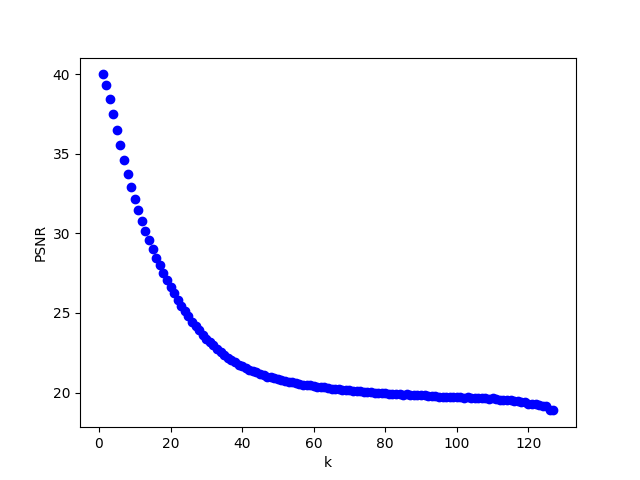
\includegraphics[width=8cm]{../imgs/output/test_psnr/k_vs_psnr.png}
\end{center}

\subsection{Variación de los parámetros}

\subsubsection{Variación del tamaño de bloque}
\label{sec:variacion_tam_bloque}

Para estudiar la variación del tamaño de bloque, se ejecutó el
algoritmo sobre las diez imágenes de prueba con el
factor de cuantización fijo en $Q = 50$,
el umbral de cuantización fijo en $U = 2000$,
y el tamaño de bloque variando con valores
$B \in \set{1,2,4,8,16,32,64,128,256,512}$.

Para cada valor de $B$, en el siguiente gráfico se muestra un
box plot de la tasa de compresión y el PSNR obtenidos:\\
\begin{center}
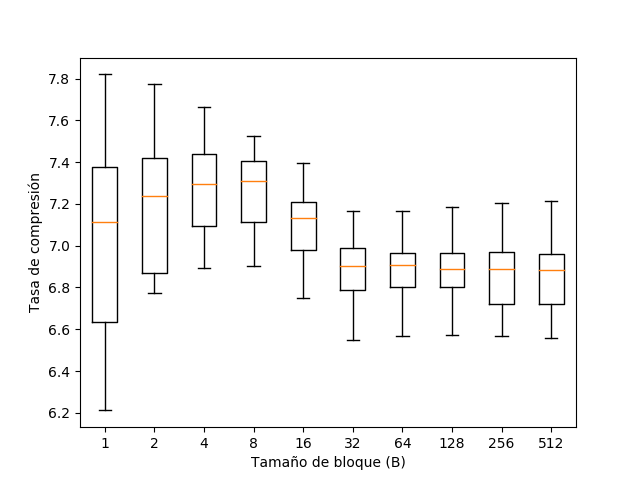
\includegraphics[width=7cm]{../imgs/output/gray_plots/b_rate.png}
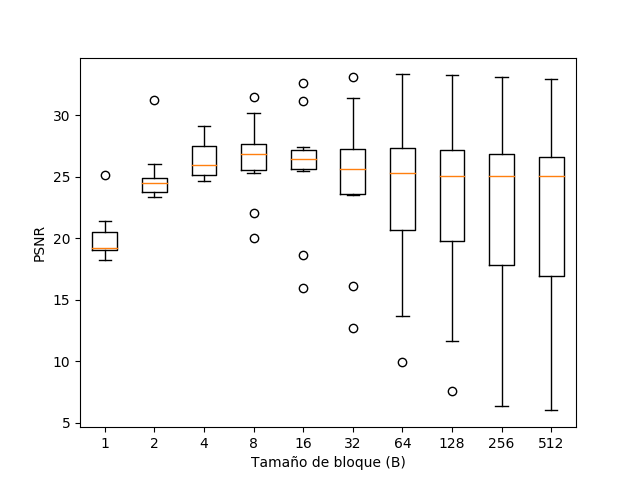
\includegraphics[width=7cm]{../imgs/output/gray_plots/b_psnr.png}
\end{center}

Puede apreciarse que hay menor varianza en la tasa de compresión
obtenida a medida que se agranda el tamaño de bloque,
mientras que hay mayor varianza en la calidad de la imagen obtenida.

Los tamaños de bloque entre $B = 4$ y $B = 16$ parecen ser razonablemente
buenos,
ya que en dichos valores se alcanza una tasa de compresión cercana a la
mejor en mediana,
y se alcanza también un valor de PSNR cercano al mejor en mediana,
con varianzas relativamente bajas.

\bigskip
En el caso límite, con tamaño de bloque $B = 1$, el proceso de
compresión no es otra cosa sino el resultado de aplicar un umbral
a los valores de gris de la imagen.
Comparar por ejemplo la siguiente imagen original con su versión
comprimida con tamaño de bloque $B = 1$:
\begin{center}
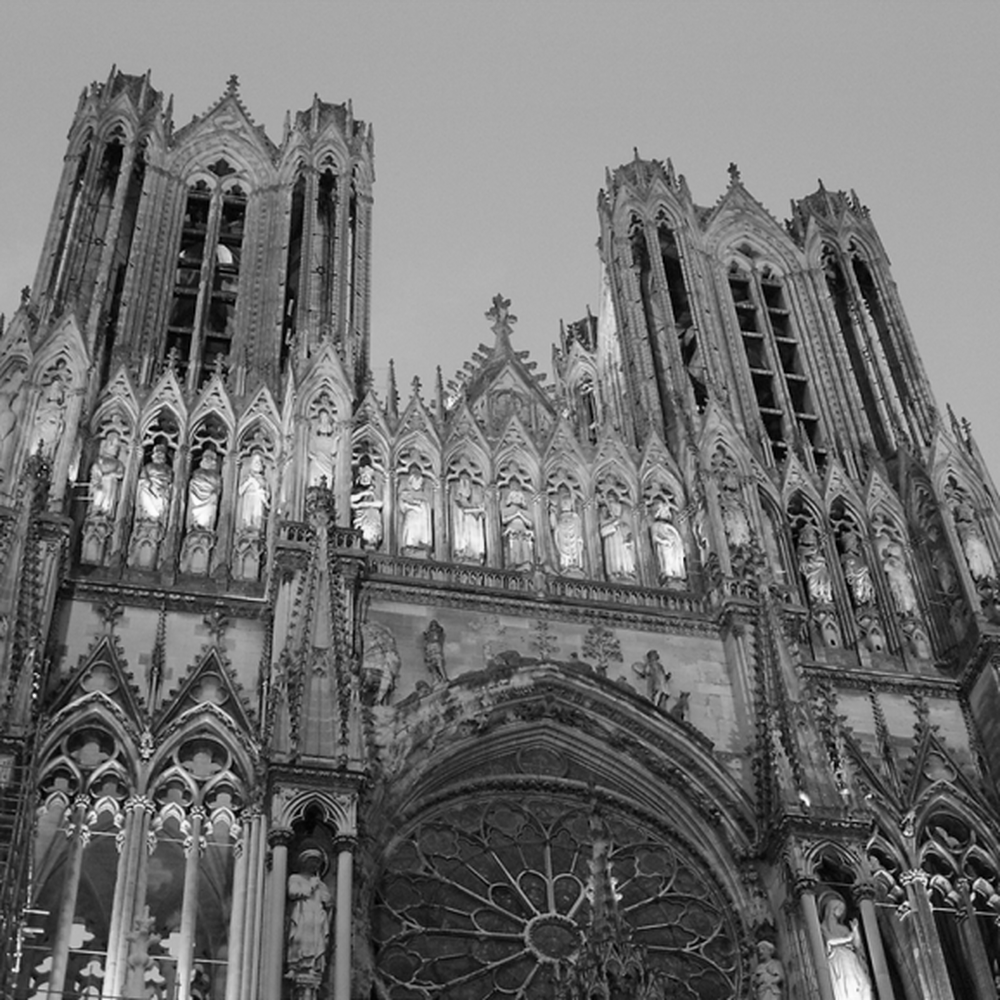
\includegraphics[width=7cm]{../imgs/input/imgs_gray/img04.png}
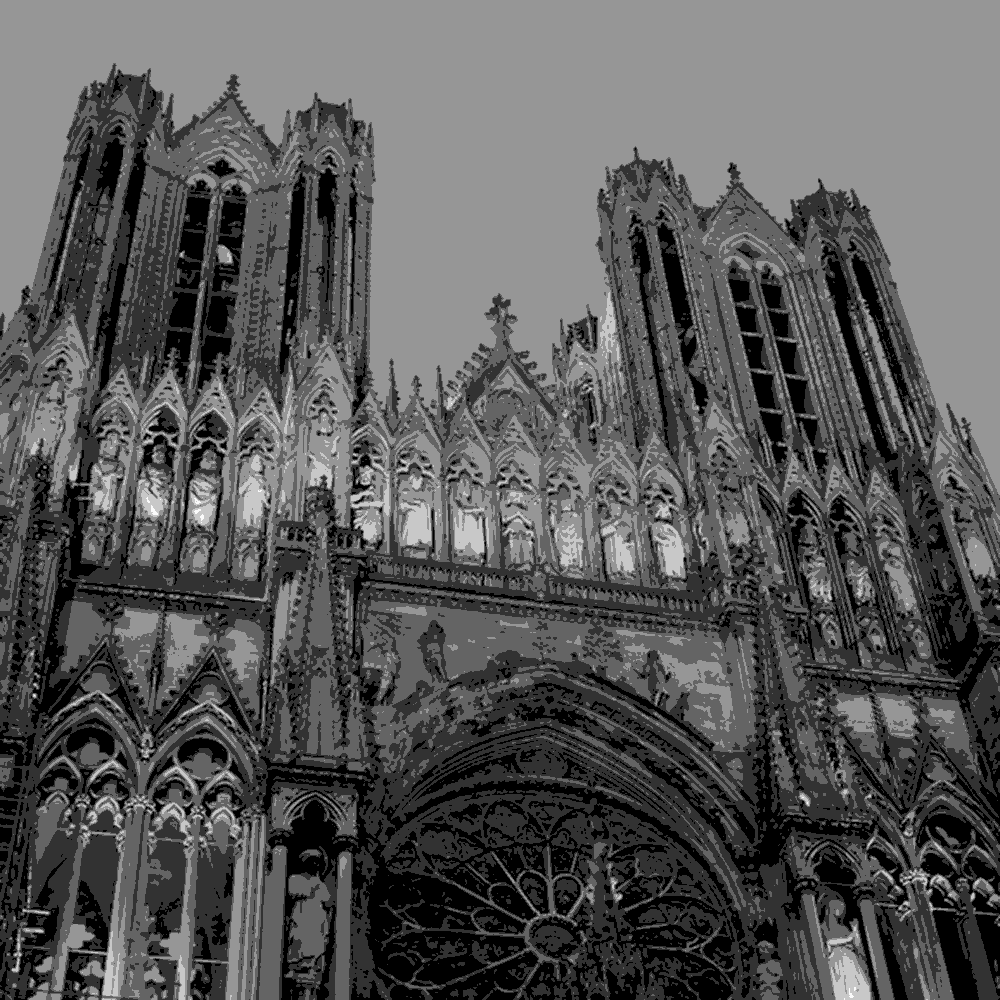
\includegraphics[width=7cm]{../imgs/output/gray_1_50_2000/img04.png}
\end{center}

\subsubsection{Variación del factor de cuantización}
\label{sec:variacion_factor_cuantizacion}

Para estudiar la variación del factor de cuantización, se ejecutó el
algoritmo sobre las diez imágenes de prueba con el
tamaño de bloque fijo en $B = 8$,
el umbral de cuantización fijo en $U = 2000$,
y el factor de cuantización variando con valores
$Q \in \set{12,25,50,100,200,400,800}$.

Para cada valor de $Q$, en el siguiente gráfico se muestra un
box plot de la tasa de compresión y el PSNR obtenidos:\\
\begin{center}
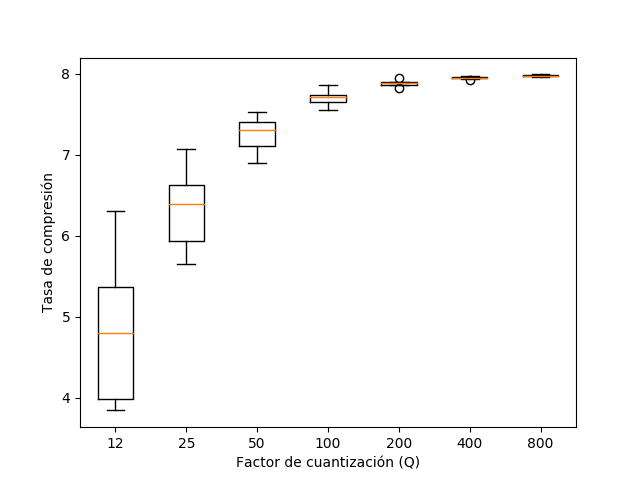
\includegraphics[width=7cm]{../imgs/output/gray_plots/q_rate.png}
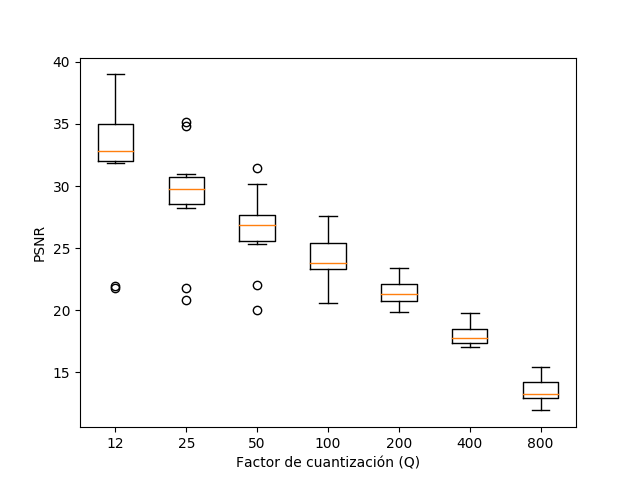
\includegraphics[width=7cm]{../imgs/output/gray_plots/q_psnr.png}
\end{center}

Como es de esperarse, la tasa de compresión aumenta a medida que
se aumenta el factor de cuantización, ya que, a mayor valor de $Q$,
los coeficientes se cuantizan en un dominio más chico.
Por otro lado, aumentar el factor de cuantización produce obviamente
una reducción en la calidad de la imagen ya que a mayor valor de $Q$
el método de compresión es más {\em lossy}.

De este modo, el parámetro $Q$ resulta útil para indicarle al método
de compresión cuál es el {\em tradeoff} que se desea establecer entre
la tasa de compresión y la calidad de la imagen.
Los editores de imagen que manipulan imágenes JPEG suelen
disponer de un control de ``nivel de compresión'' deseado, que
se obtiene a cambio de una menor calidad.

\subsubsection{Variación del umbral de cuantización}

Para estudiar la variación del umbral de cuantización, se ejecutó el
algoritmo sobre las diez imágenes de prueba con el
tamaño de bloque fijo en $B = 8$,
el factor de cuantización fijo en $Q = 50$,
y el umbral de cuantización variando con valores
$U \in \set{31, 62, 125, 250, 500, 1000, 2000, 4000, 8000, 16000}$.

Para cada valor de $U$, en el siguiente gráfico se muestra un
box plot de la tasa de compresión y el PSNR obtenidos:\\
\begin{center}
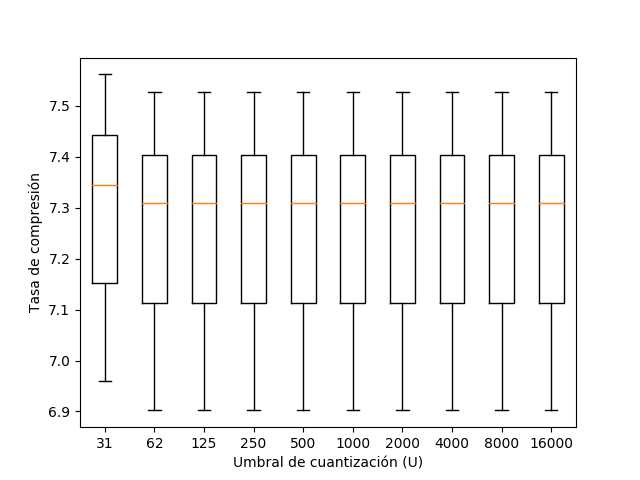
\includegraphics[width=7cm]{../imgs/output/gray_plots/u_rate.png}
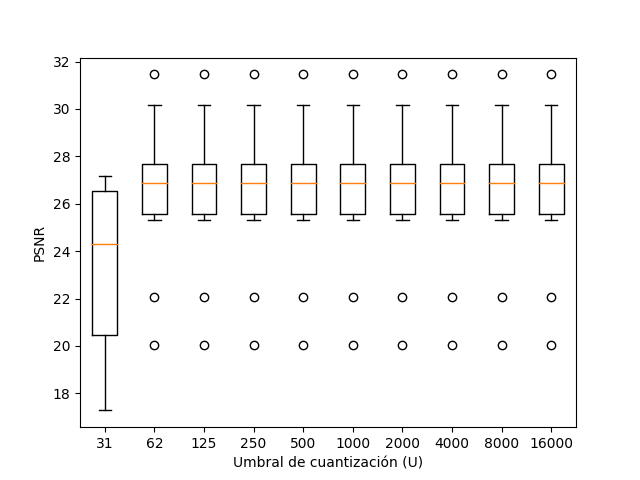
\includegraphics[width=7cm]{../imgs/output/gray_plots/u_psnr.png}
\end{center}

No se encuentran diferencias significativas para valores de $U$
superiores a 31 en el rango de valores elegido.
Esto sugiere que el rango en el que se hizo variar el valor del
parámetro $U$
está mal elegido.
Se repitió el análisis para el rango de valores
$U \in \set{5, 10, 15, 20, 25, 30, 35, 40, 45, 50}$.
\begin{center}
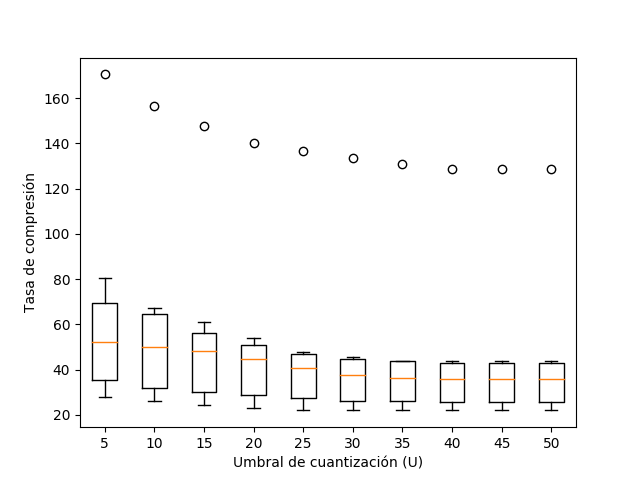
\includegraphics[width=7cm]{../imgs/output/gray_plots/ualt_rate.png}
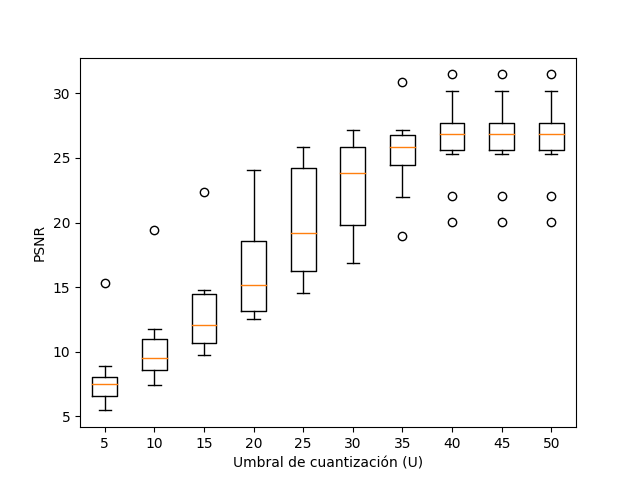
\includegraphics[width=7cm]{../imgs/output/gray_plots/ualt_psnr.png}
\end{center}
En este rango sí es posible apreciar, como es de esperarse, que
a medida que aumenta el valor de $U$,
la tasa de compresión disminuye e, inversamente, la calidad de
la imagen aumenta.

\subsection{Elección de parámetros}

A efectos de elegir ``buenos parámetros'', se fijó
el tamaño de bloque en $B = 8$. Esta elección se justifica con las
observaciones realizadas en la Sección~\ref{sec:variacion_tam_bloque}.

\subsubsection{Elección del factor de cuantización $Q$}

A continuación, se buscó un valor de $Q$ ``razonable''.
Como ya se mencionó en la Sección~\ref{sec:variacion_factor_cuantizacion},
es imposible seleccionar un valor de $Q$ universal, ya que esta
decisión depende del {\em tradeoff} que se quiera establecer entre
la tasa de compresión y la calidad de la imagen.
(En el caso límite, si la calidad de la imagen es de carácter fundamental,
no correspondería utilizar un compresor {\em lossy}).

No obstante, se intentó fijar un valor $Q$ ``razonable''.
Para ello nos concentramos en la medida de PSNR asociada al valor de $Q$.
Visualmente, un valor de PSNR superior a $30$dB resulta consistentemente aceptable,
mientras que un valor inferior a $20$dB resulta consistentemente inaceptable.
Se ejecutó nuevamente el método de compresión sobre las imágenes de prueba.
Como objetivo nos propusimos un valor de $Q$ que alcance un PSNR de al menos $20$dB
para todas las imágenes, y con mediana mayor a $30$dB.
De acuerdo con lo estudiado en la
Sección~\ref{sec:variacion_factor_cuantizacion}
este valor se hallaría aproximadamente entre $Q = 1$ y $Q = 25$.
Se hizo variar nuevamente $Q$ entre dichos valores.
Para realizar esta búsqueda, se fijó el umbral $U$ en un valor
muy grande ($U = 10^6$),
para evitar que este parámetro tenga algún tipo de incidencia en el resultado.

Los box plots para la tasa de compresión y el PSNR
asociados a estas ejecuciones se pueden ver en los siguientes gráficos:
\begin{center}
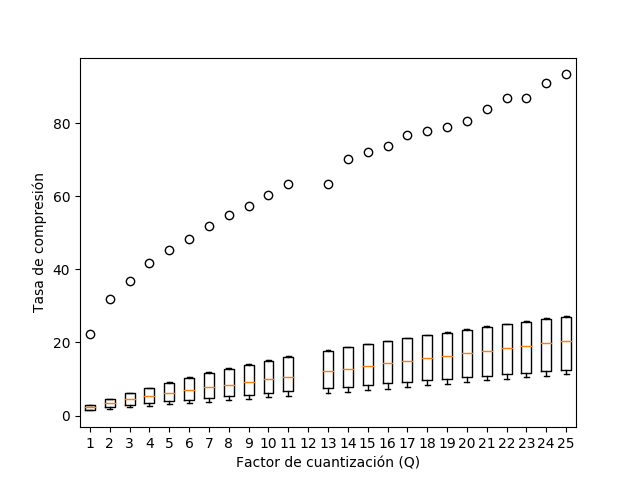
\includegraphics[width=7cm]{../imgs/output/gray_plots/qalt_rate.png}
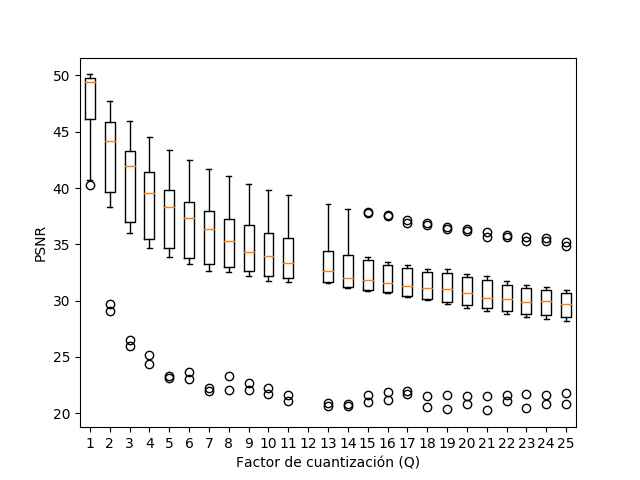
\includegraphics[width=7cm]{../imgs/output/gray_plots/qalt_psnr.png}
\end{center}

Este experimento vuelve a validar que, a medida que varía $Q$,
el comportamiento del método varía de forma relativamente ``continua'',
y por lo tanto no hay un único valor universal correcto para $Q$,
sino que se trata de un {\em tradeoff}, sumamente dependiente del
contexto de aplicación.

Por otro lado, el valor del factor de cuantización $Q = 25$
parece razonable,
ya que alcanza tasas de compresión de un orden de magnitud
(entre 10 y 20 aproximadamente), manteniendo el PSNR sobre 30
de manera consistente.

La peor calidad se alcanza en el caso de imágenes con bordes delineados,
como la siguiente, que presenta numerosas manifestaciones del {\em ringing effect},
y una tasa de compresión de $40 : 1$.

\begin{center}

\includegraphics[width=4cm]{../imgs/input/imgs_gray/img00.png}
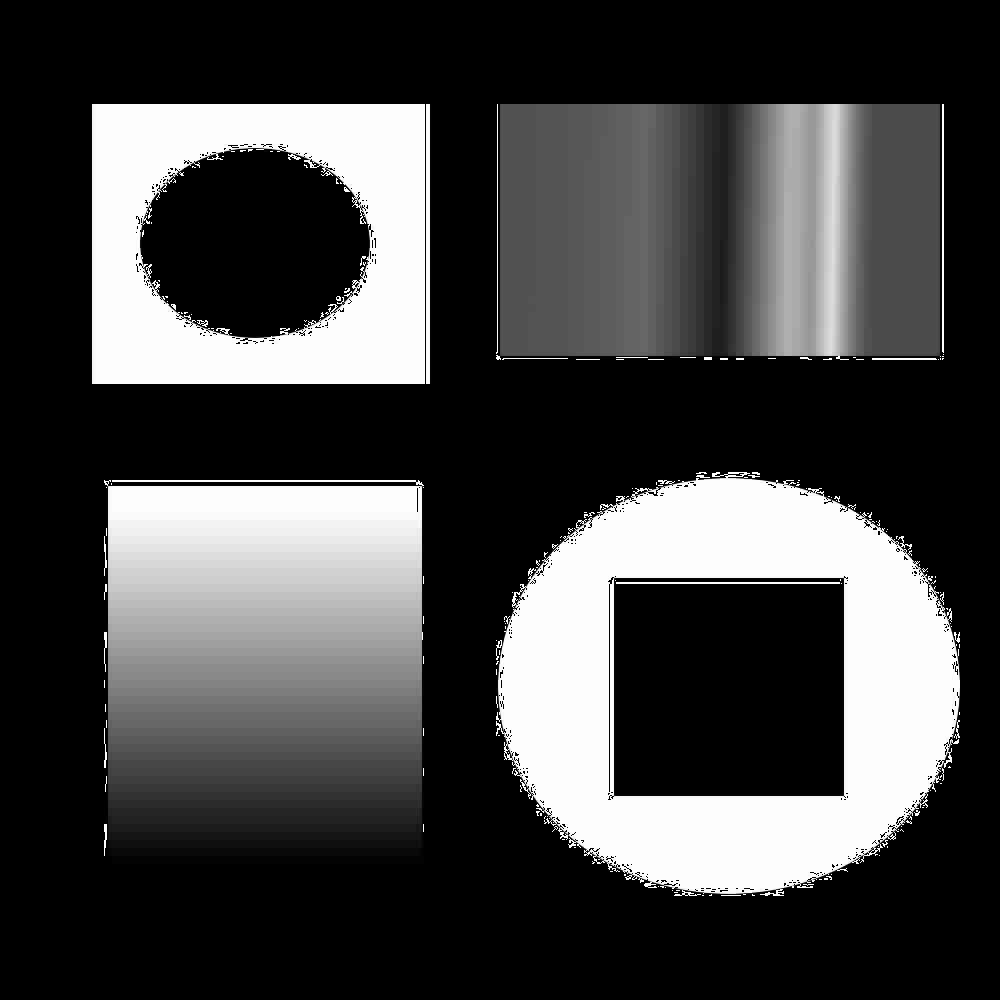
\includegraphics[width=4cm]{../imgs/output/gray_8_25_1000000/img00.png}
\end{center}

En el otro extremo, la mejor calidad se alcanza en el caso
de una fotografía ``típica'', en la cual la calidad visual es excelente
(con manifestaciones del {\em blocking effect} inapreciables a primera vista),
y una tasa de compresión no negligible de $2.47 : 1$:

\begin{center}
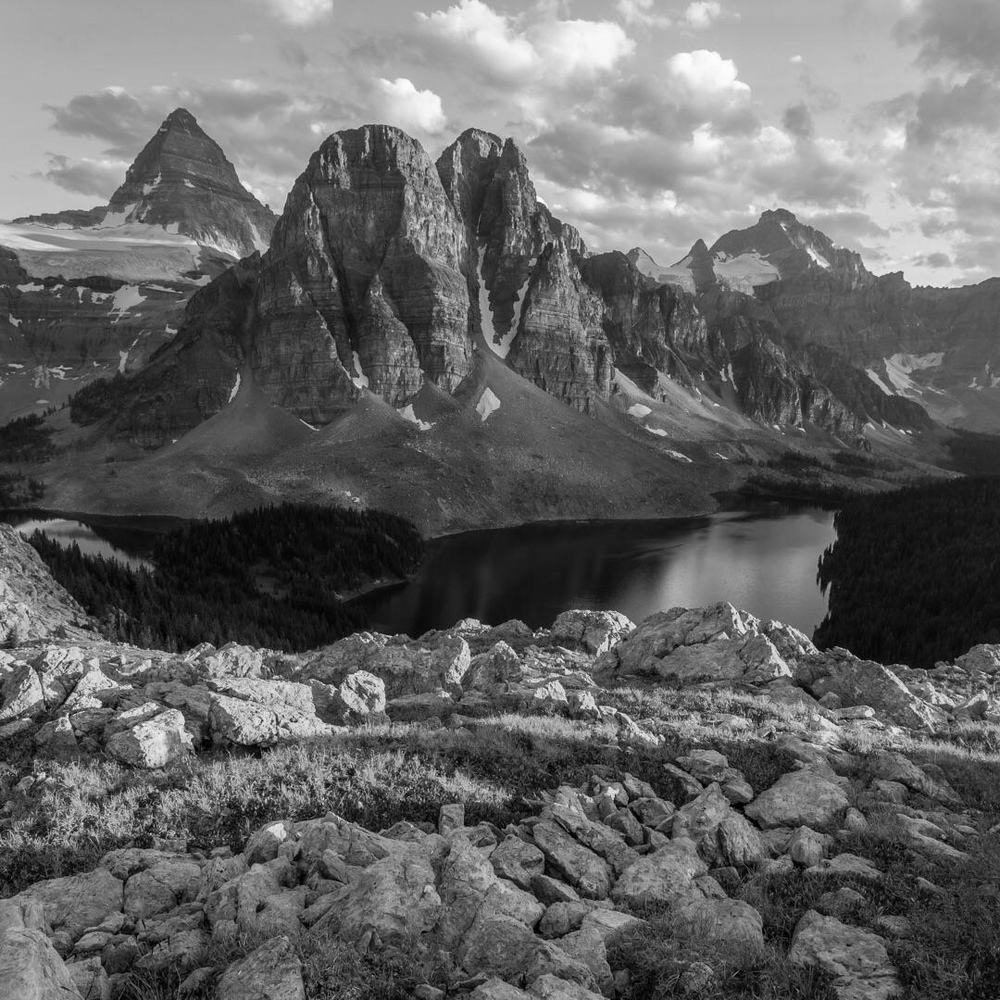
\includegraphics[width=4cm]{../imgs/input/imgs_gray/img01.png}
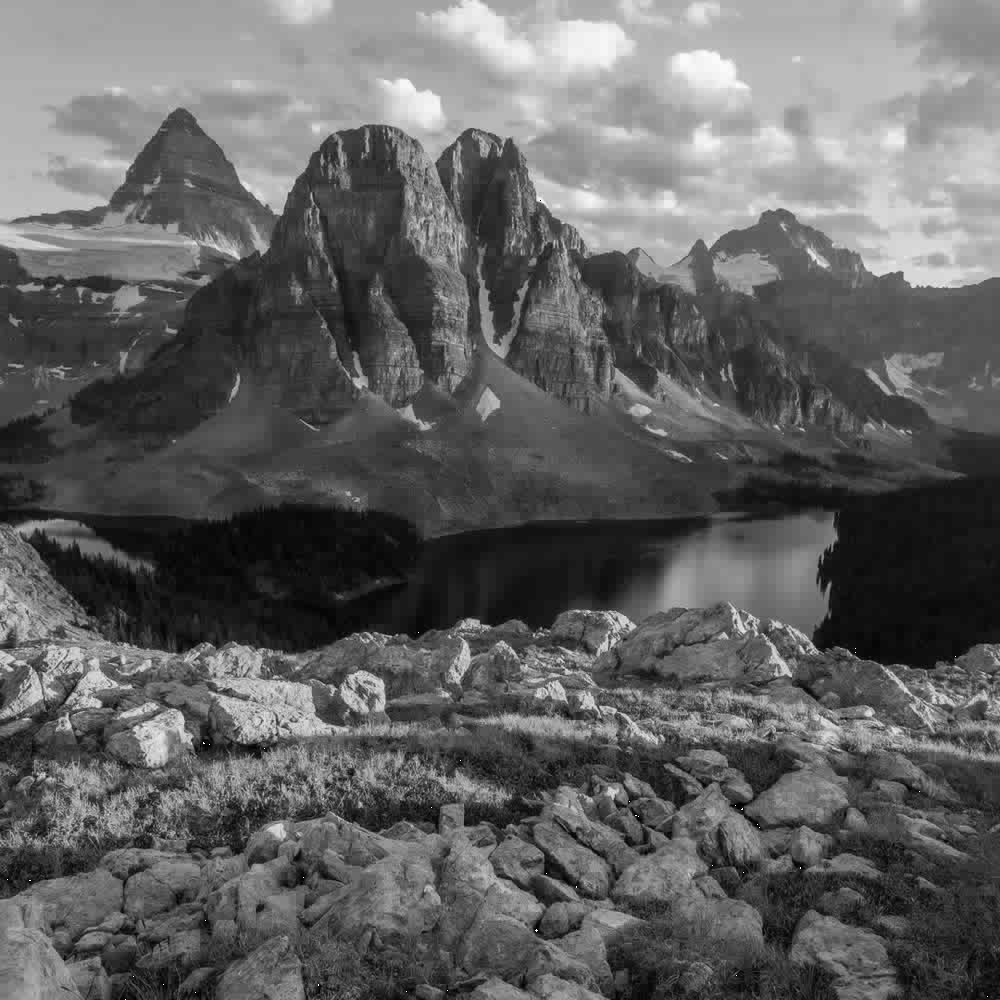
\includegraphics[width=4cm]{../imgs/output/gray_8_25_1000000/img01.png}
\end{center}

\subsubsection{Elección del umbral de cuantización $U$}

\TODO{TODO}

\section{Variantes del método}

\subsection{Transmisión progresiva}

Tal vez la forma maś intuitiva de llegar a tener una transmisión progresiva de una imágen es simplemente dividirla por bloques y enviarlos serialmente a través de la red. El problema con esta técnica es que el tiempo de carga puede ser muy mala en imágenes que tarden en transmitirse: sólo podemos mostrar las partes de la imágen que ya recibimos, y por ende siempre hay una parte que estaría ``en blanco''.

El estandard de JPEG propone lo que el comité denomina ``progressive mode''. Este consiste en ir transmitiendo los coeficientes de la DCT para todos los bloques, llenando la cantidad de coeficientes por bloque a medida que pasa el tiempo. Por ejemplo, podríamos primero enviar todos los coeficientes DC, luego los primeros AC, y así sucesivamente.

Queda claro que al agregar coeficientes la imágen se iría volviendo cada vez más nítida, ya que tendríamos más información para aproximarla. Esto reduce ampliamente el problema de las ``áreas en blanco'' al cargar la imagen: sólo precisaríamos los primeros coeficientes de cada bloque para tener una aproximación razonable mientras que terminamos de cargar la imagen.

Hay múltiples formas de decidir exactamente qué enviar; las dos ideas más simples son enviar una cantidad limitada de coeficientes y enviar una aproximación de los coeficientes en lugar de los valores reales. Qué coeficientes enviar puede también realizarse de múltiples formas: el recorrido zig-zag que vimos anteriormente, una submatriz superior, los de mayor valor absoluto, etcétera. El paper referido por el enunciado~[1] recomienda seguir el orden zig-zag e ir agregando bits menos significativos en cada transmisión.

Cabe destacar que esto es ampliamente utilizado en la práctica (basta con utilizar un browser sobre una conexión lenta para darse cuenta), ya que en general el bottleneck de cualquier aplicación que transmite información a través de una red está precisamente en la entrada y salida, más que en el uso de CPU.

No realizamos una implementación de esto por no tener suficiente tiempo para experimentar, pero ambas implementaciones realizadas son fácilmente extensibles para lograr este propósito: basta con agregar un buffer entre el código responsable de quantizar, y el código responsable de hacer entropy coding; este buffer sería leído cuando se desee enviar la imágen, y se correría entropy coding de alguna forma sobre el mismo antes de enviarlo.

\subsection{Matriz de factores de cuantización}

En general, es esperable que los coeficientes de la DCT de menor frecuencia
sean más relevantes que los coeficientes de menor frecuencia
para representar una imagen con mayor fidelidad.
Es por ello que una posible mejora al método de compresión es no utilizar el
mismo factor $Q$ para todos los coeficientes de un bloque, sino utilizar
distintos factores.

Se implementó una variante del método para tamaño de bloque $B = 8$ con la
matriz dada por:
\[
  Q_{ij} = 20 \cdot i \cdot j
\]
Así, al coeficiente de frecuencia más baja (coeficiente DC)
le corresponde un factor de $Q_{1,1} = 20$,
mientras que al coeficiente de frecuencia más alta
le corresponde un factor de $Q_{8,8} = 1280$.
\medskip

En los siguientes dos gráficos se comparan la tasa de compresión y PSNR obtenidos
para el método de referencia (con $Q = 50$ fijo, representado con puntos azules),
así como la tasa de compresión y PSNR obtenidos
para el método con $Q$ variable (con los coeficientes dados por la matriz $Q$
de arriba, representado con cruces rojas).
En ambos casos el eje $x$ corresponde a cada una de las diez imágenes de prueba.
\begin{center}
  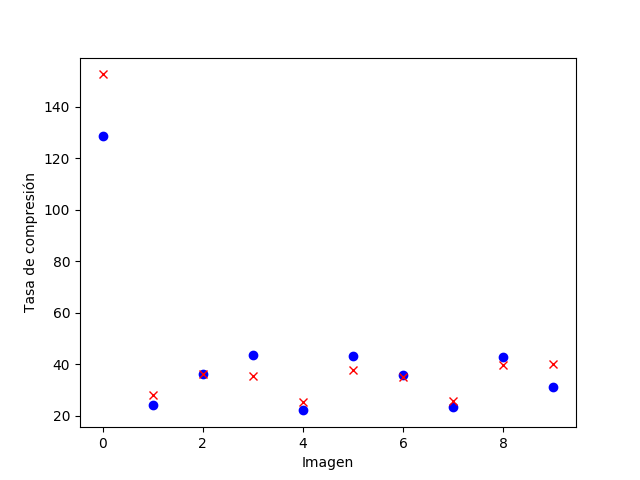
\includegraphics[width=7cm]{../imgs/output/qmatrix_plots/qmatrix_rate.png}
  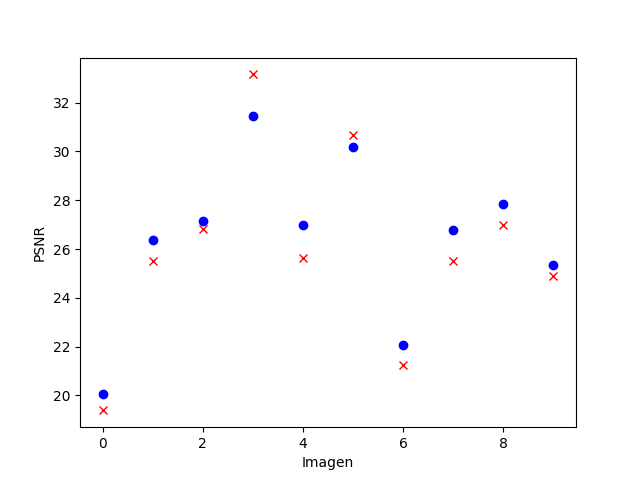
\includegraphics[width=7cm]{../imgs/output/qmatrix_plots/qmatrix_psnr.png}\\
  {\bf Comparación entre los métodos con $Q$ fijo y con $Q$ variable}
\end{center}

No se aprecia una diferencia significativa entre los dos métodos,
resultando similares tanto en la tasa de compresión como en la calidad
de las imágenes obtenida.

Se ensayó el mismo experimento también con otras matrices $Q$.
En ningún caso se encontró un comportamiento claramente superador del método
original.

\subsection{{\em Wavelet transform}}

  \TODO{TODO}

\section{Conclusiones}

\TODO{TODO}

\newpage
\appendix
\section{Imágenes de prueba en tonos de gris}

\subsection{Imágenes originales}

\begin{figure}[!htp]
\begin{center}
\begin{tabular}[t]{|ll|ll|ll|}
\hline
img0 & 
\includegraphics[width=3cm]{../imgs/input/imgs_gray/img00.png} &
img1 & 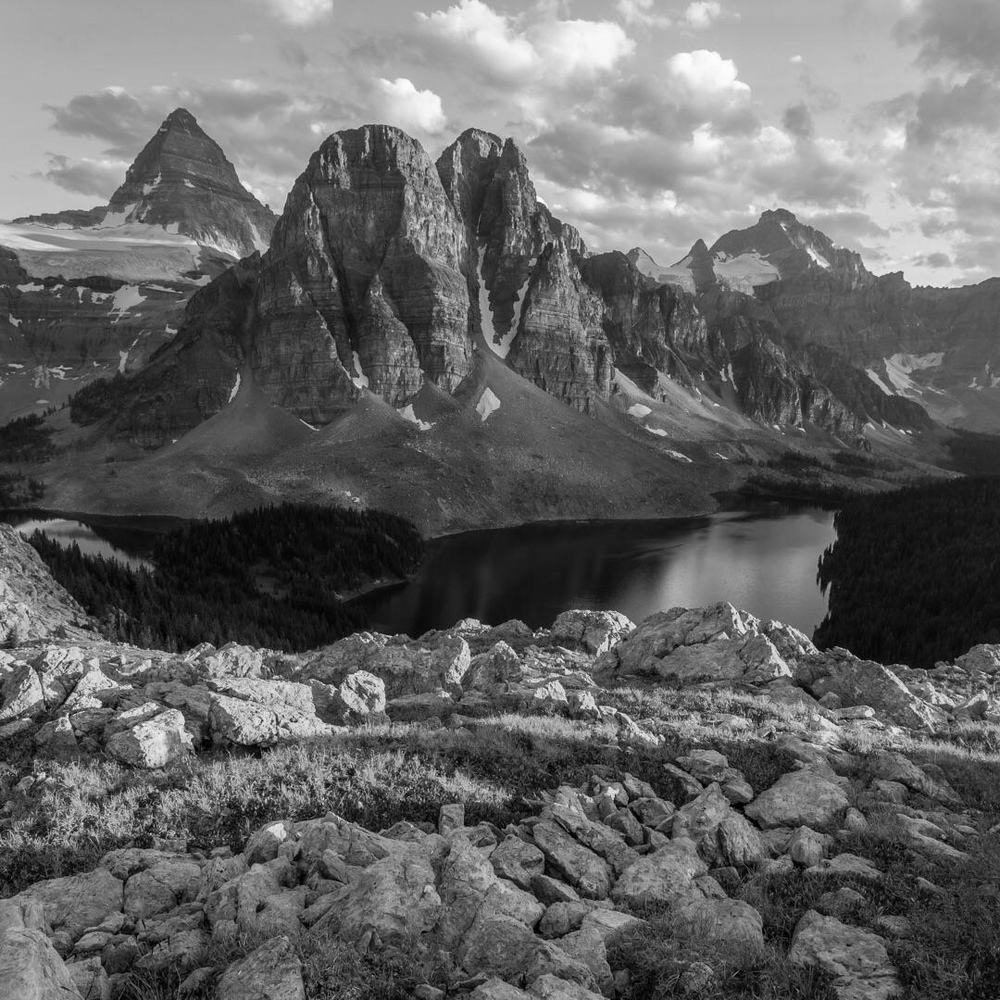
\includegraphics[width=3cm]{../imgs/input/imgs_gray/img01.png} &
img2 & 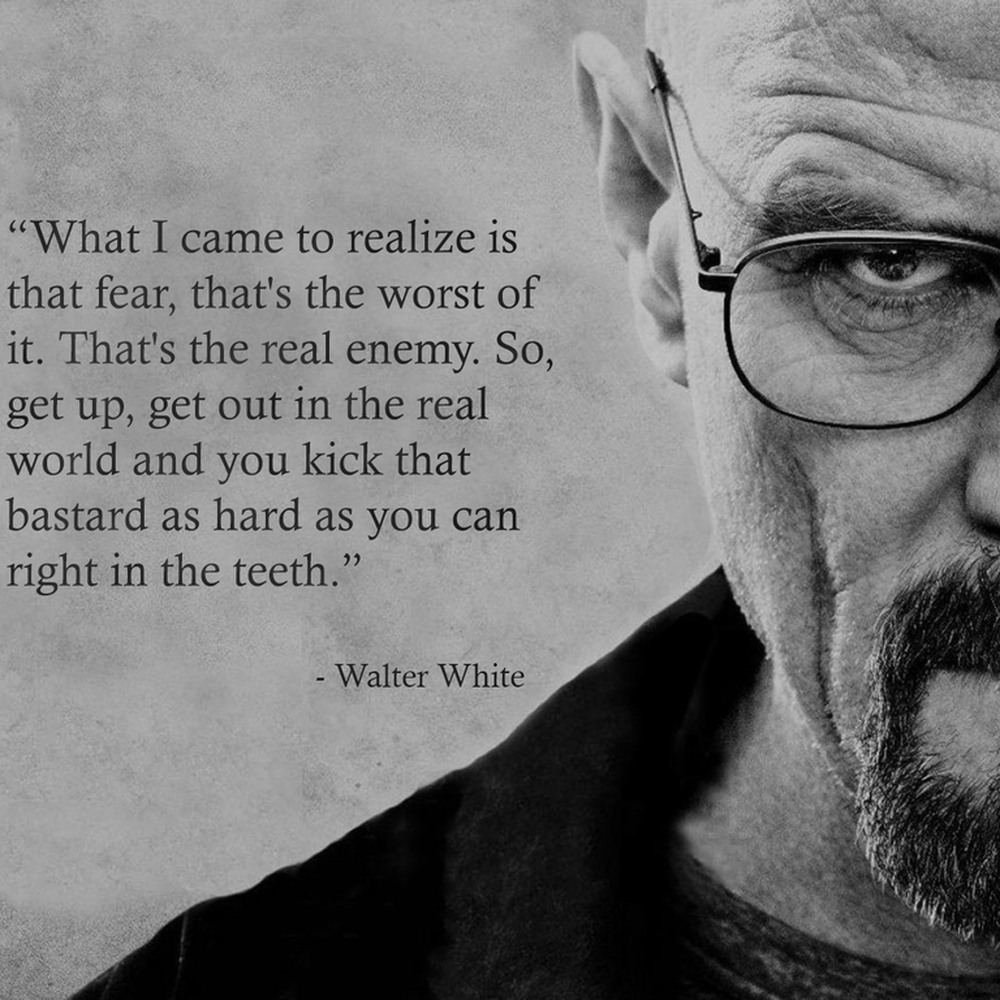
\includegraphics[width=3cm]{../imgs/input/imgs_gray/img02.png} \\
\hline
img3 & 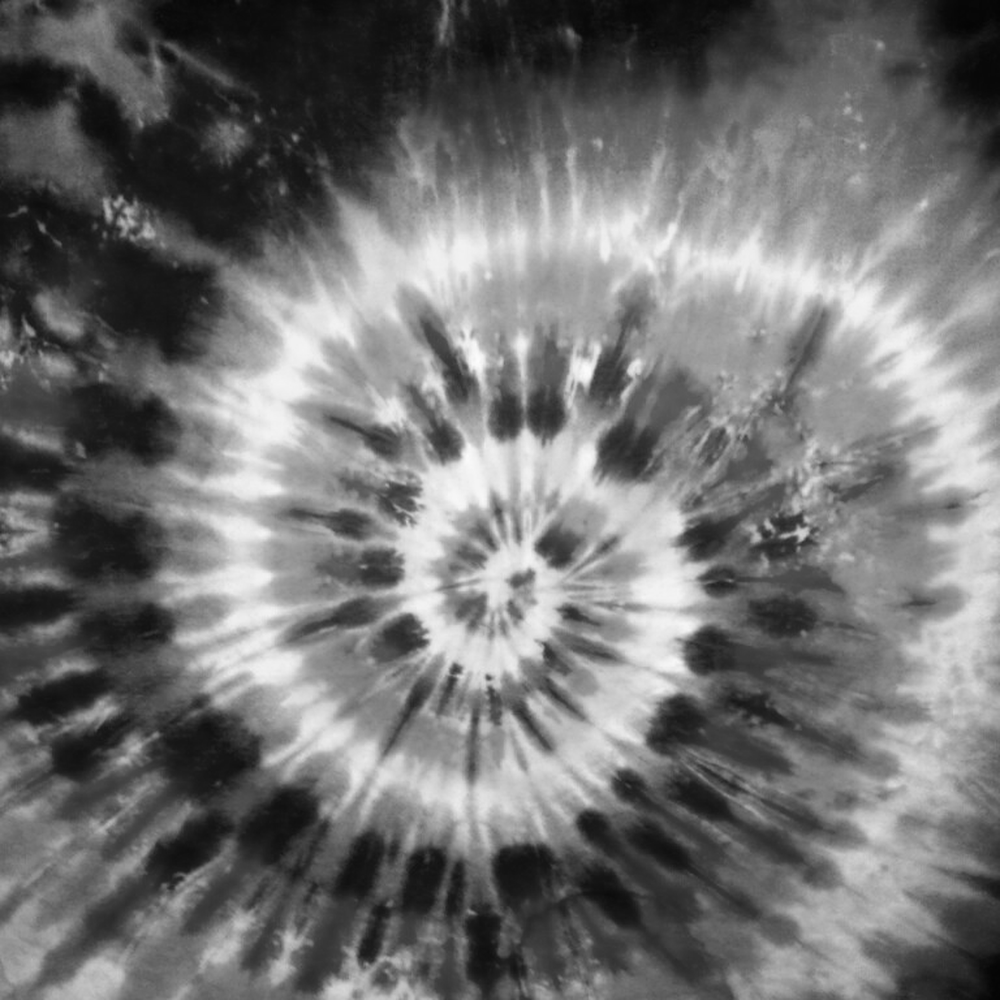
\includegraphics[width=3cm]{../imgs/input/imgs_gray/img03.png} &
img4 & 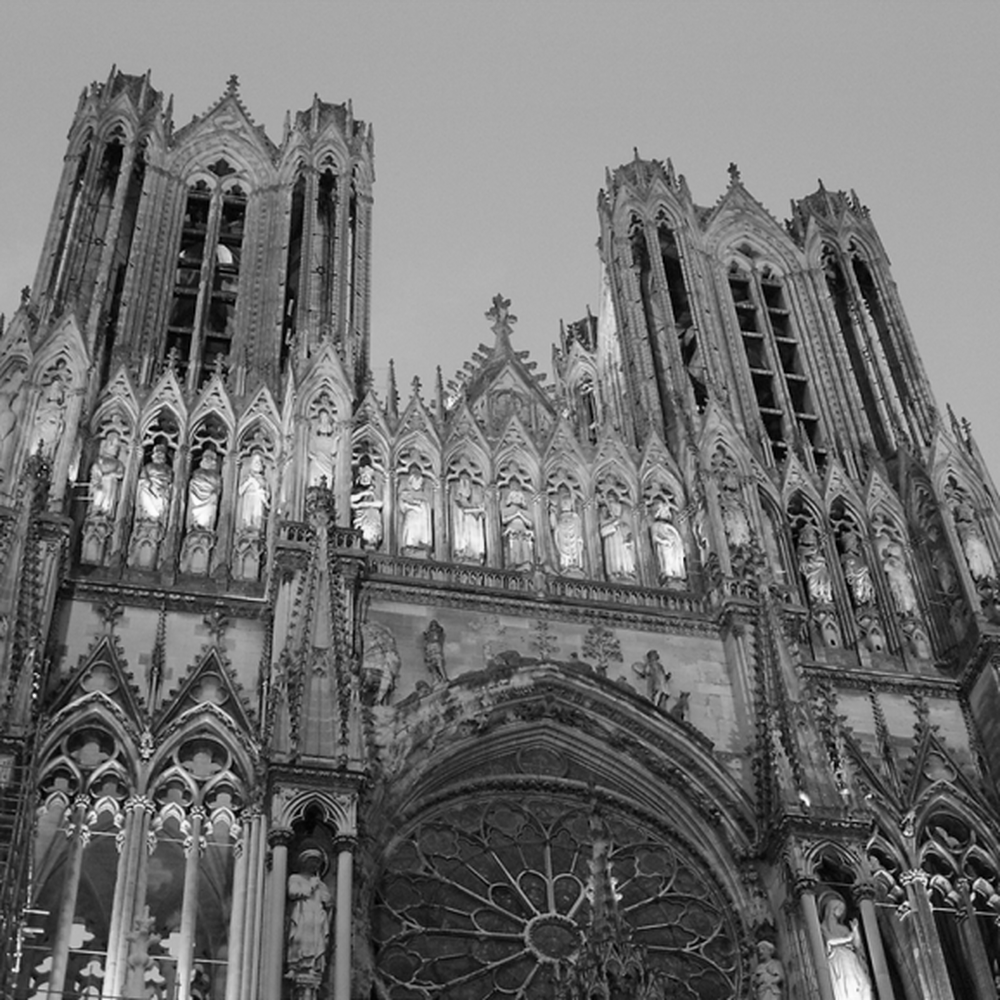
\includegraphics[width=3cm]{../imgs/input/imgs_gray/img04.png} &
img5 & 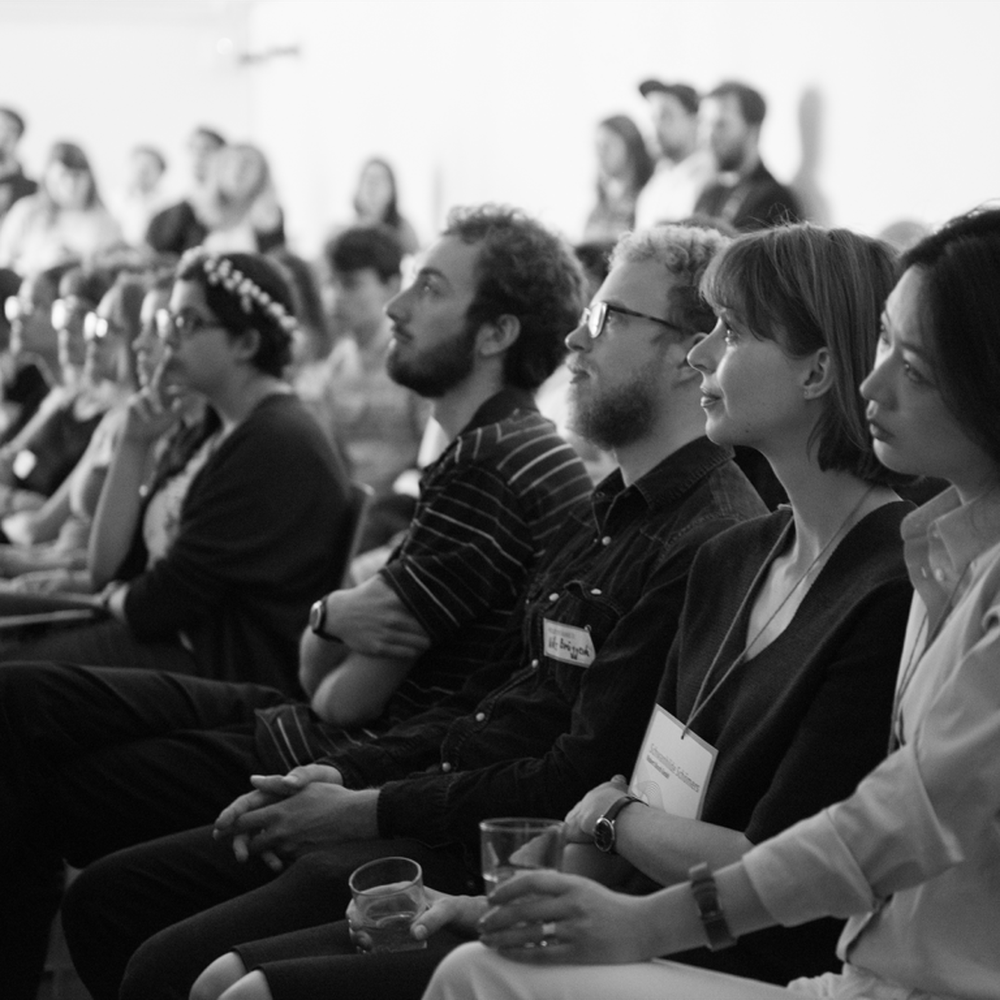
\includegraphics[width=3cm]{../imgs/input/imgs_gray/img05.png} \\
\hline
img6 & 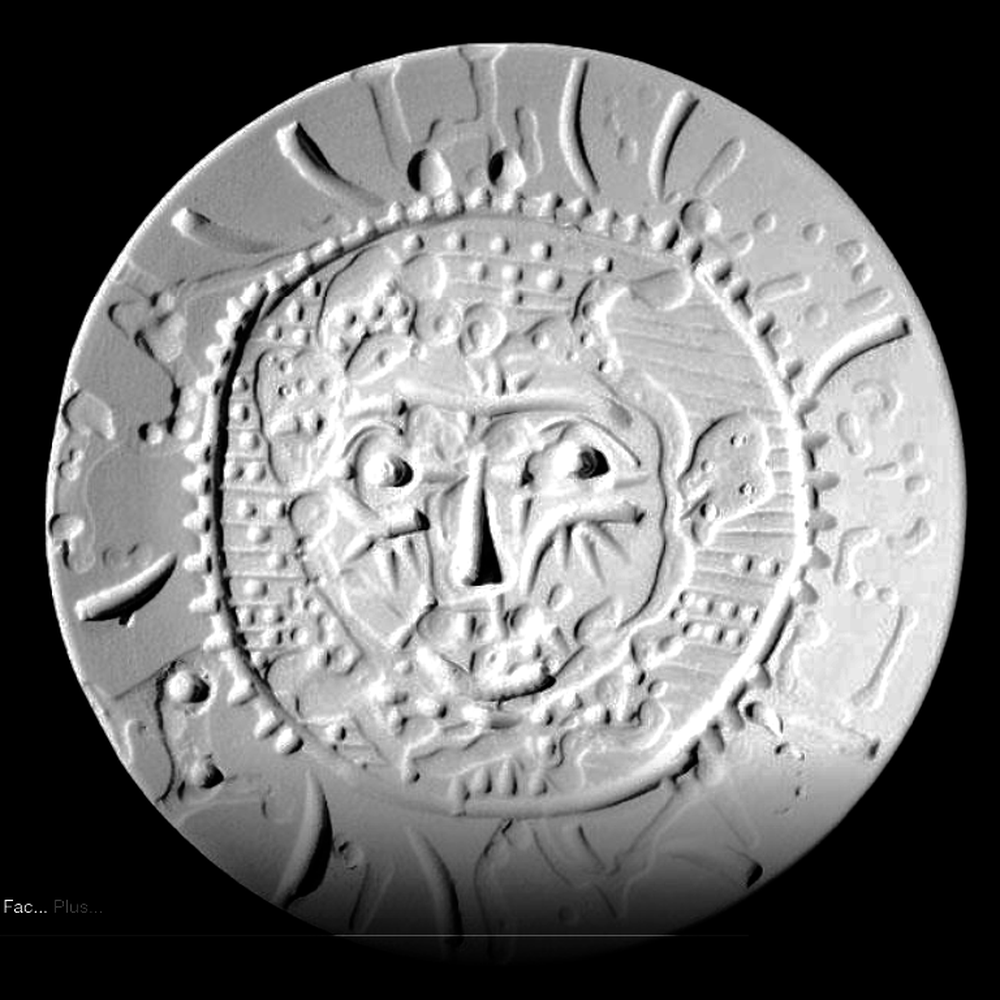
\includegraphics[width=3cm]{../imgs/input/imgs_gray/img06.png} &
img7 & 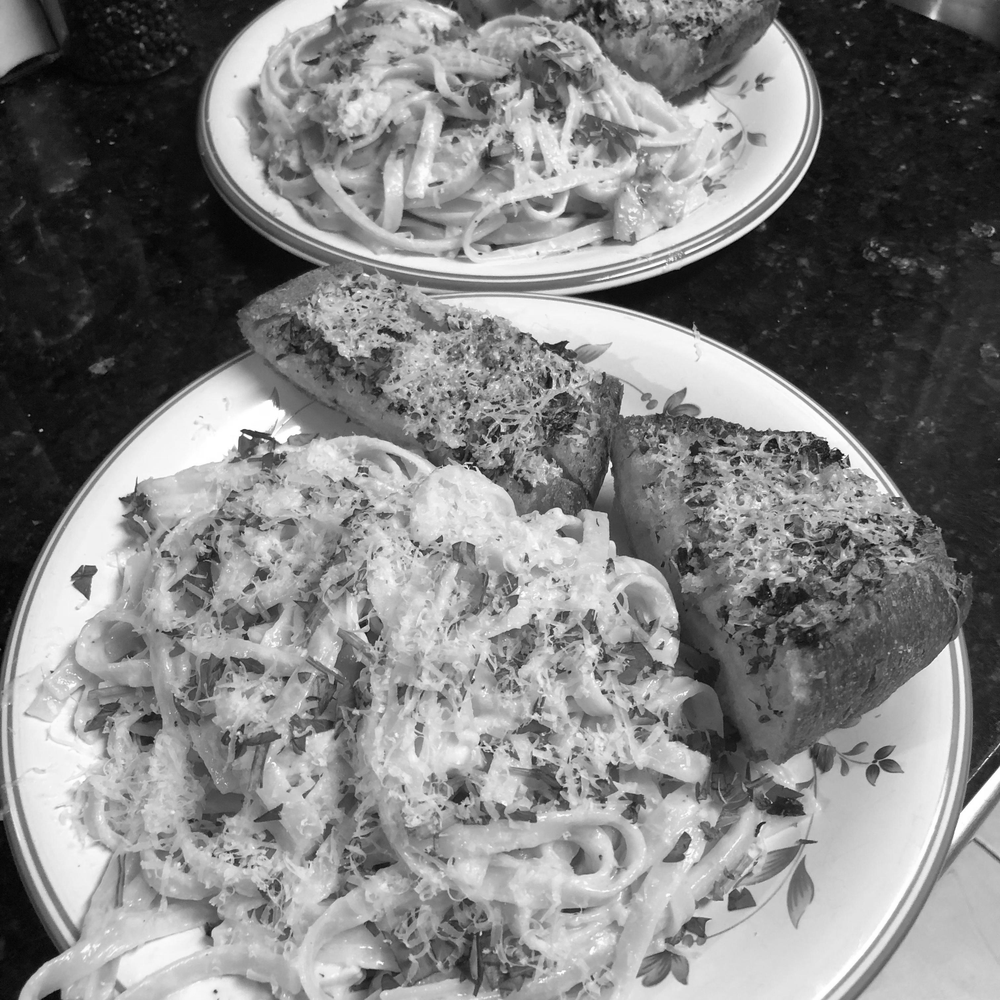
\includegraphics[width=3cm]{../imgs/input/imgs_gray/img07.png} &
img8 & 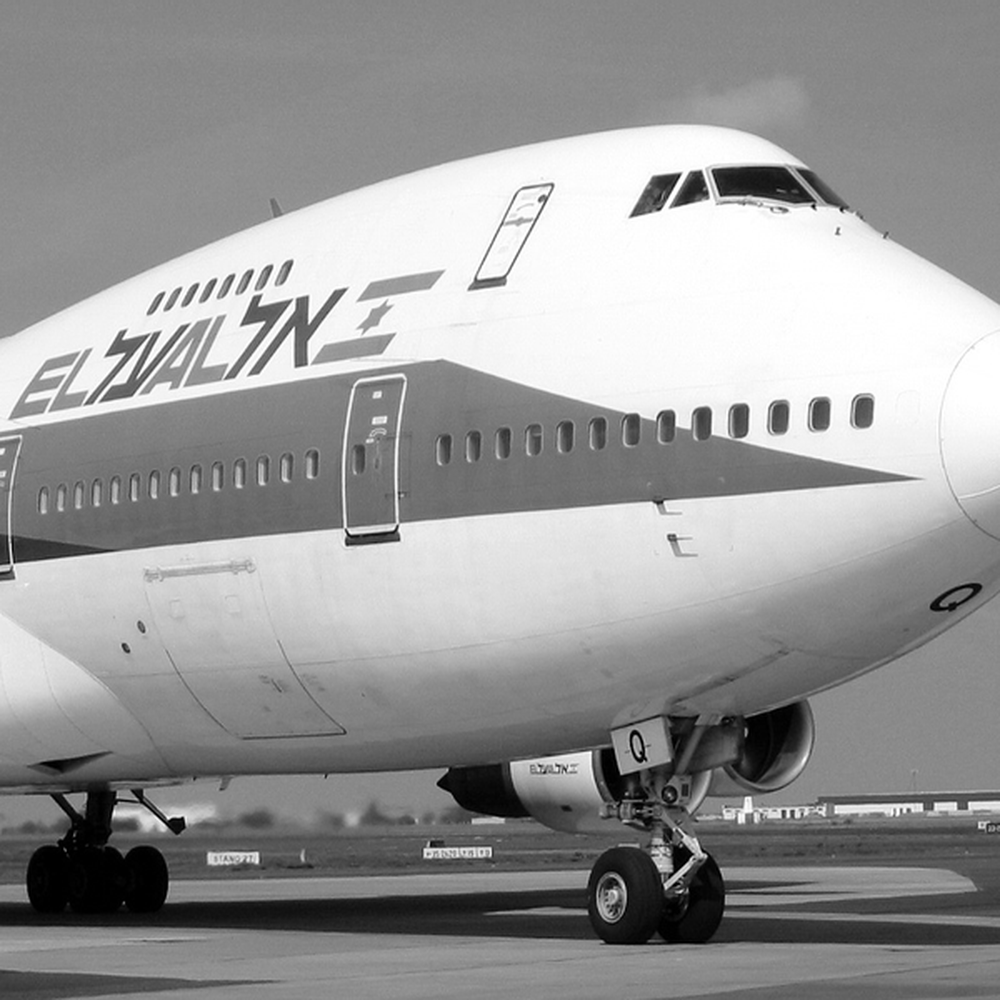
\includegraphics[width=3cm]{../imgs/input/imgs_gray/img08.png} \\
\hline
img9 & 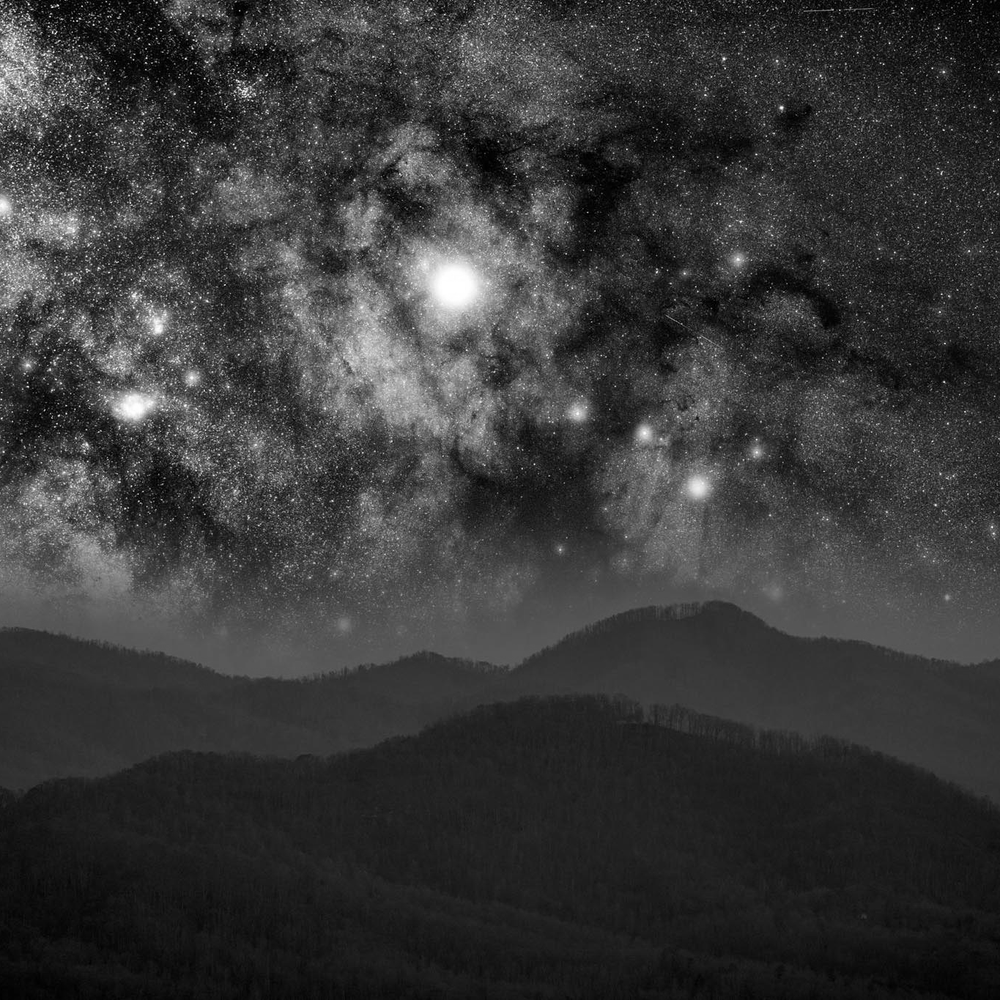
\includegraphics[width=3cm]{../imgs/input/imgs_gray/img09.png} &&&& \\
\hline
\end{tabular}
\end{center}
\caption{Imágenes de prueba en tonos de gris}
\label{fig:imagenes_de_prueba_gris}
\end{figure}

\newpage
\subsection{Imágenes comprimidas}

\begin{figure}[!htp]
\begin{center}
\begin{tabular}[t]{|ll|ll|ll|}
\hline
img0 & 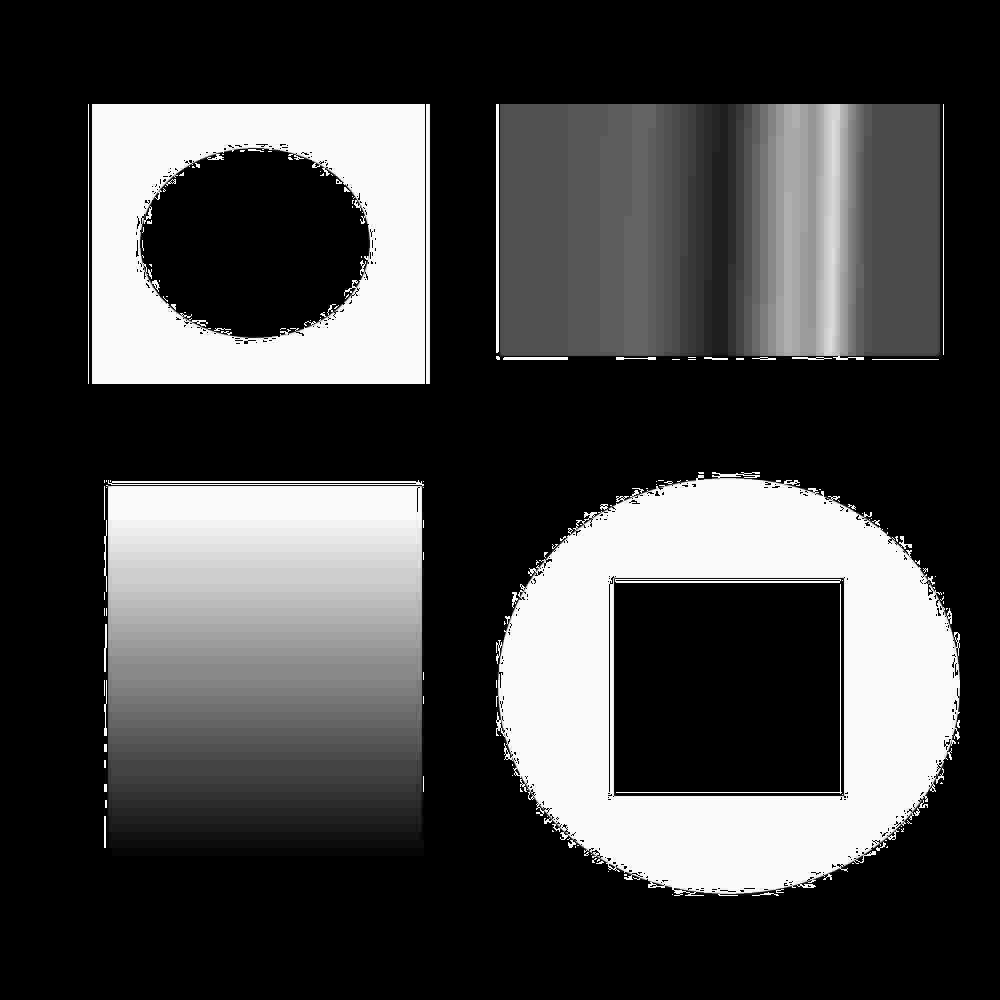
\includegraphics[width=3cm]{../imgs/output/gray_8_50_2000/img00.png} &
img1 & 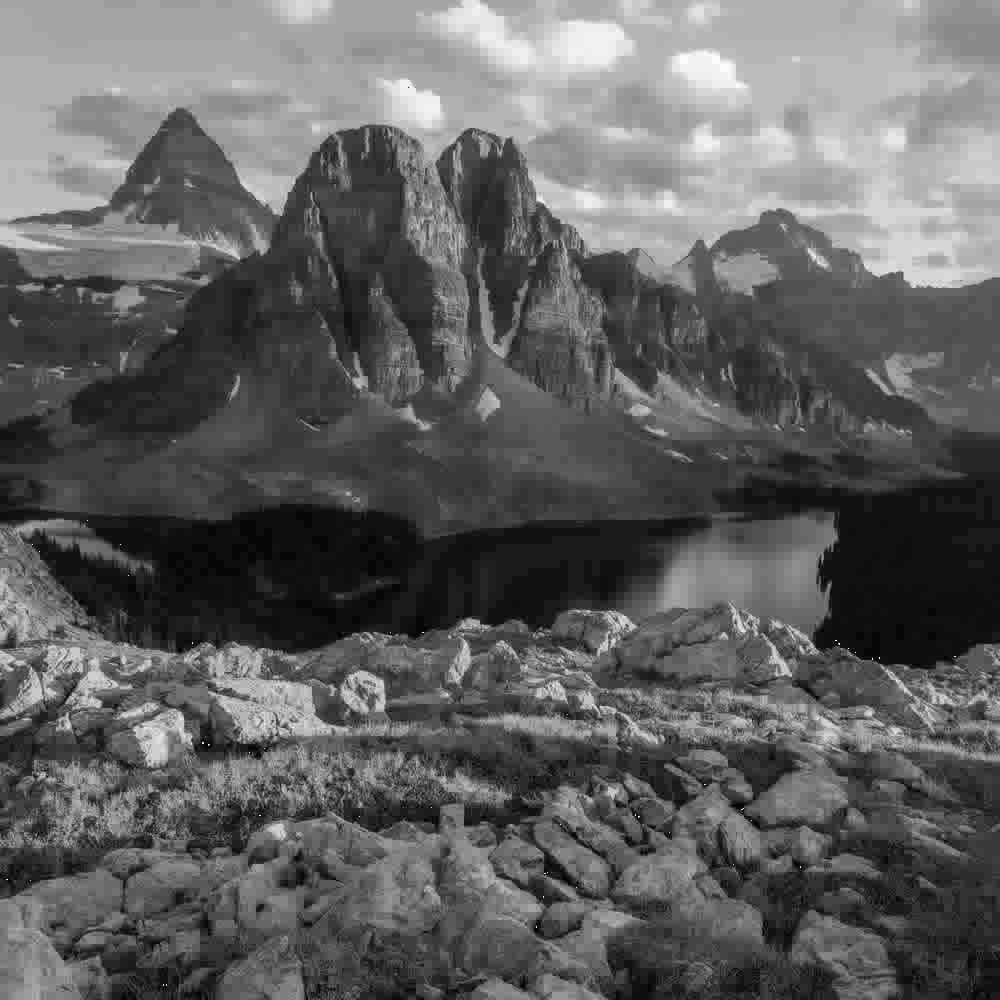
\includegraphics[width=3cm]{../imgs/output/gray_8_50_2000/img01.png} &
img2 & 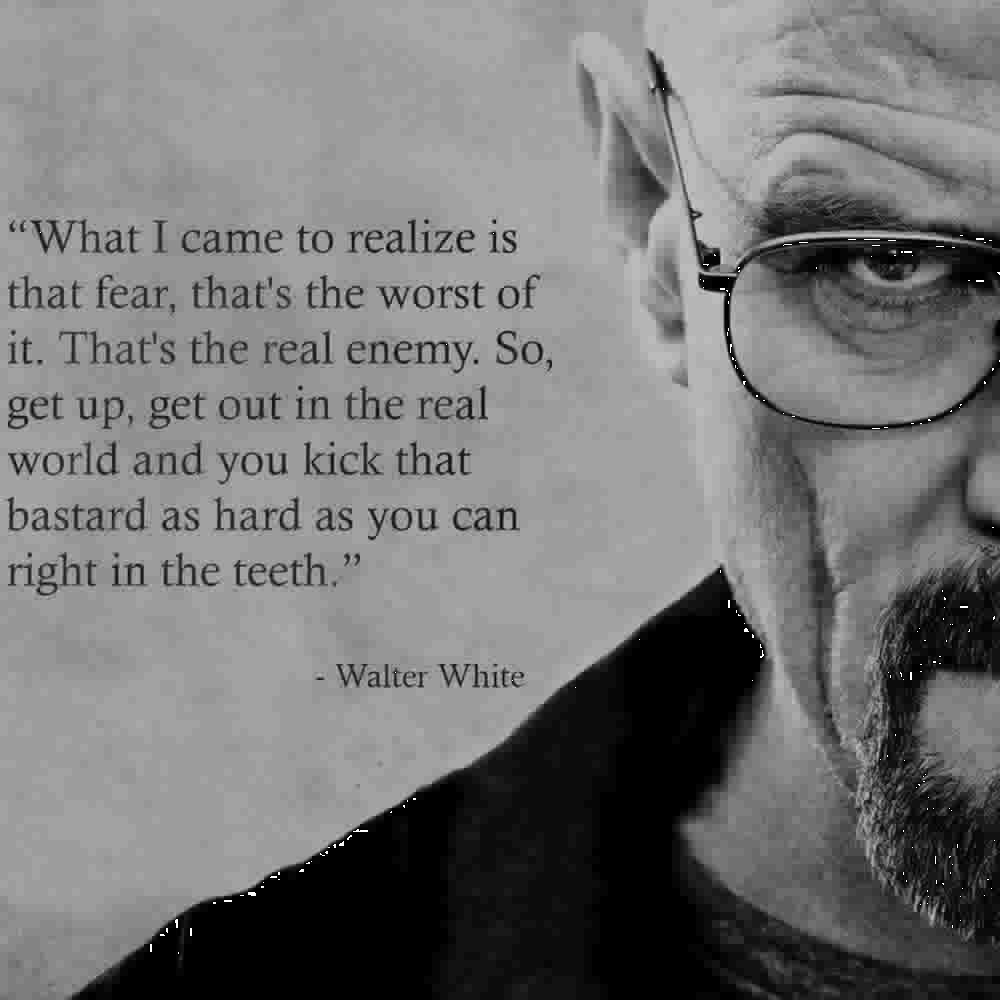
\includegraphics[width=3cm]{../imgs/output/gray_8_50_2000/img02.png} \\
\hline
img3 & 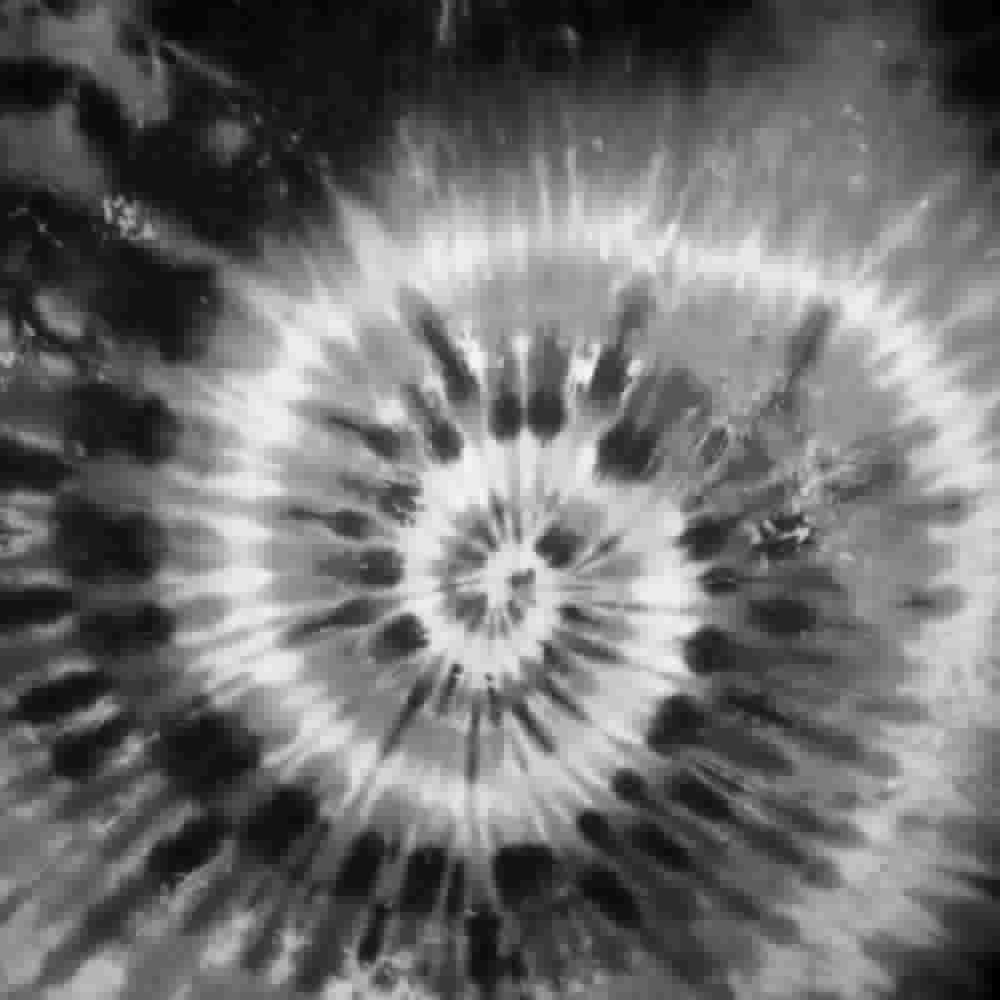
\includegraphics[width=3cm]{../imgs/output/gray_8_50_2000/img03.png} &
img4 & 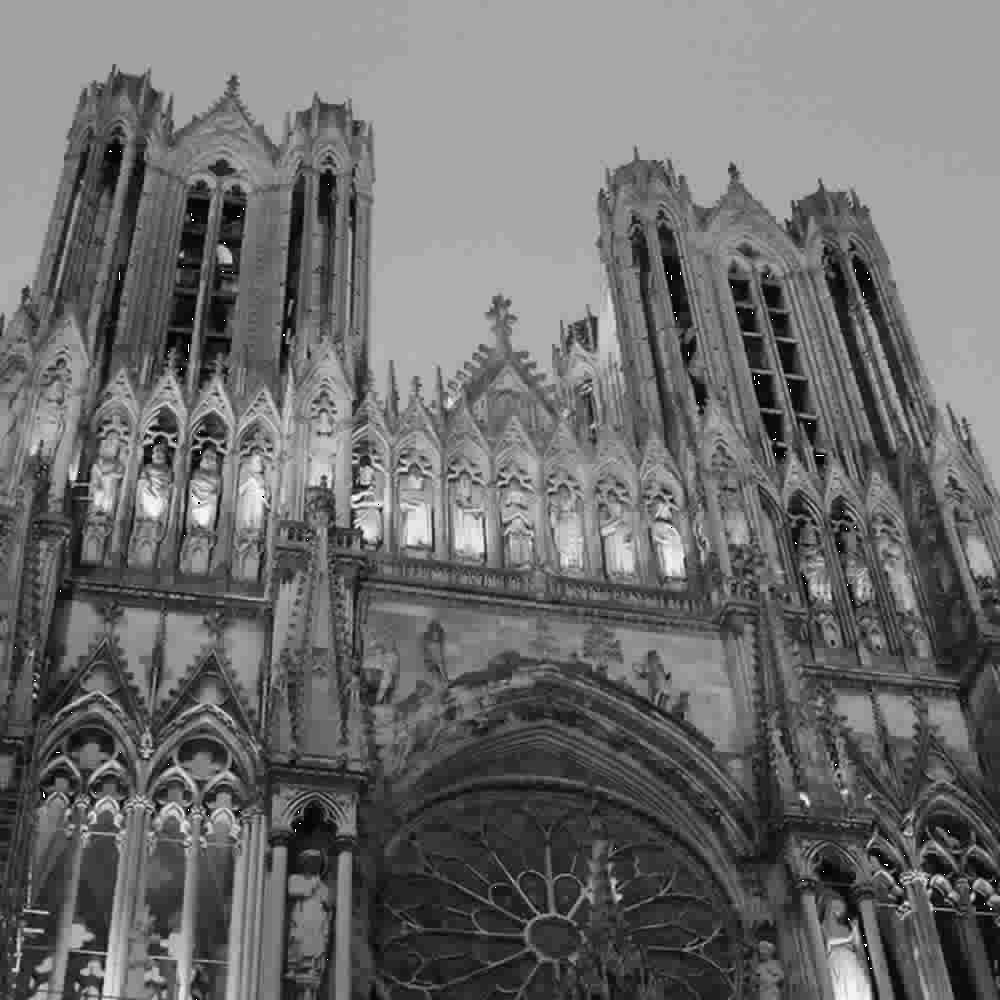
\includegraphics[width=3cm]{../imgs/output/gray_8_50_2000/img04.png} &
img5 & 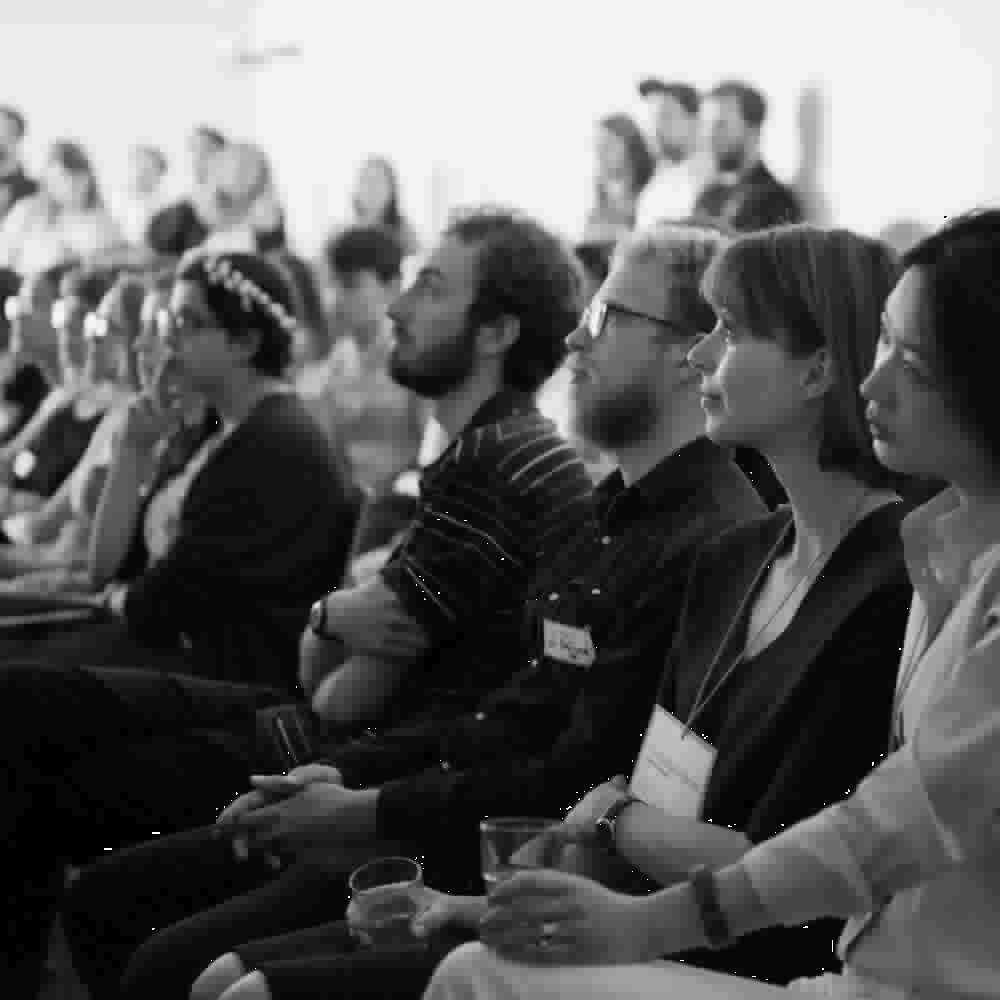
\includegraphics[width=3cm]{../imgs/output/gray_8_50_2000/img05.png} \\
\hline
img6 & 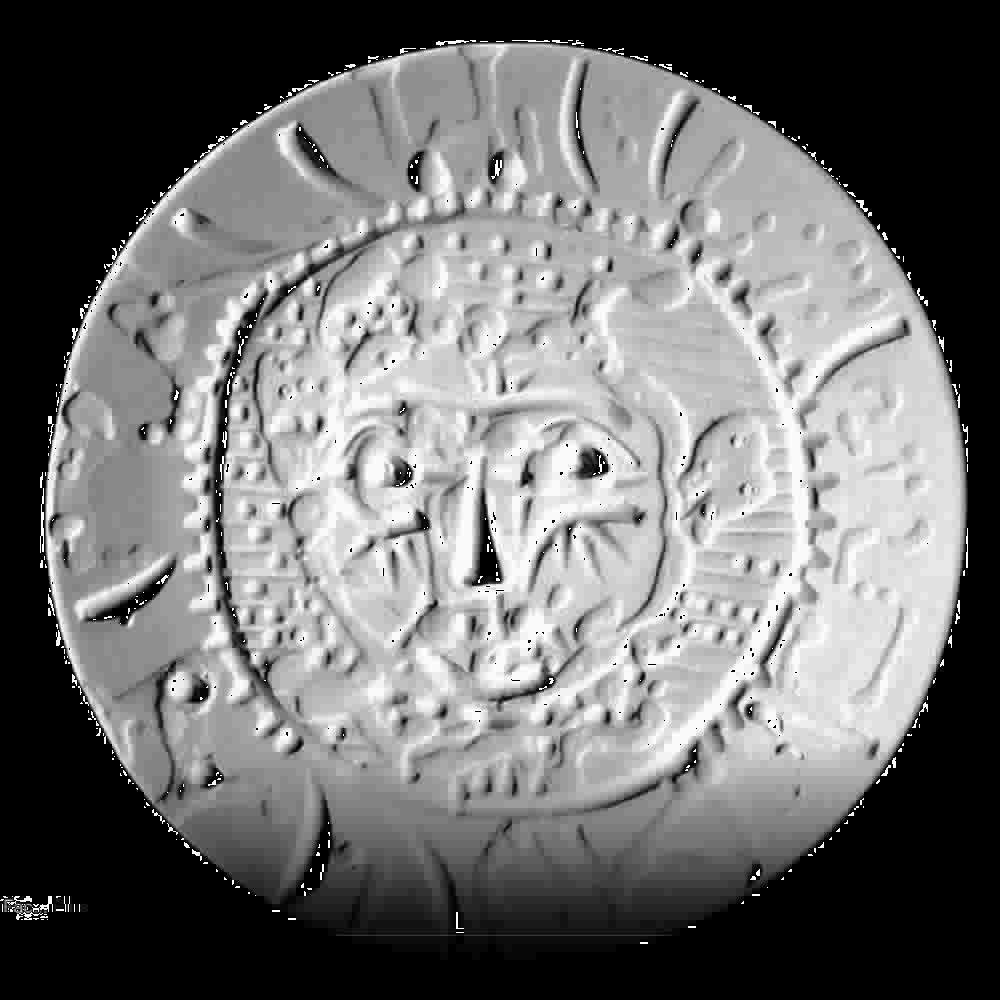
\includegraphics[width=3cm]{../imgs/output/gray_8_50_2000/img06.png} &
img7 & 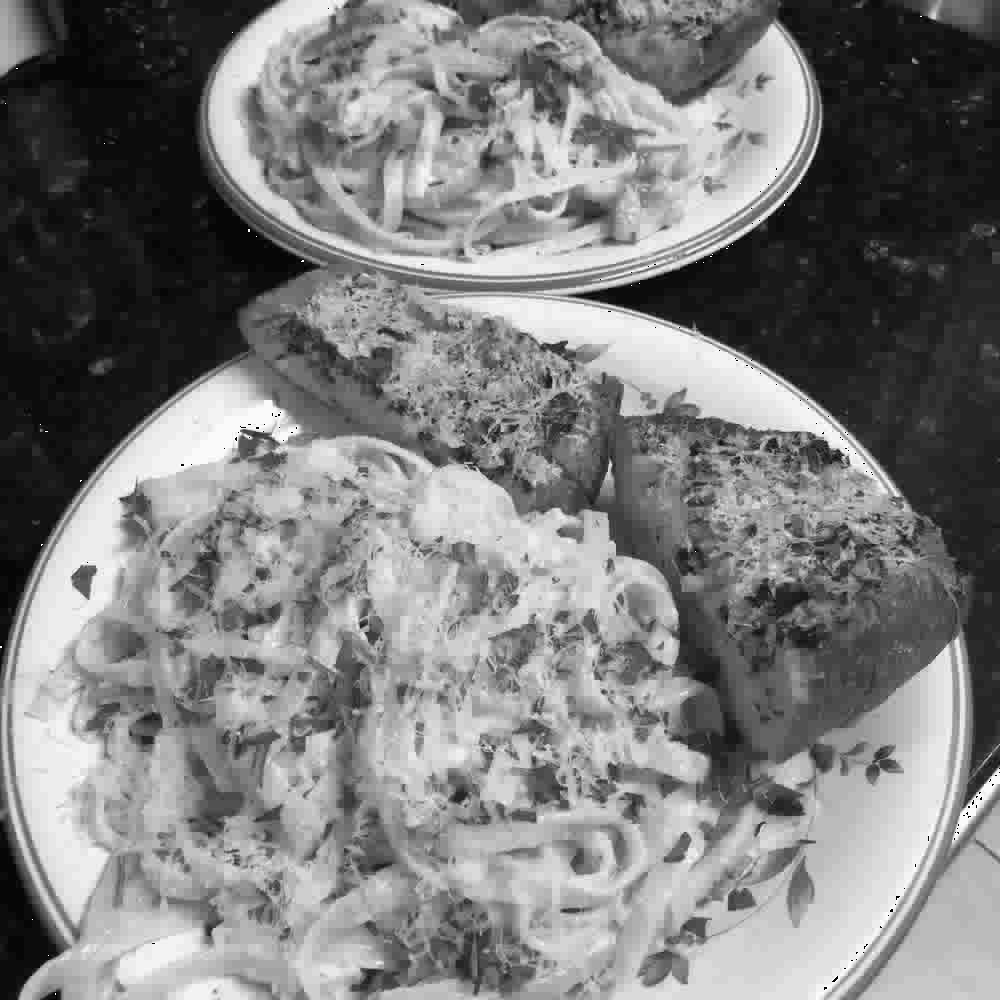
\includegraphics[width=3cm]{../imgs/output/gray_8_50_2000/img07.png} &
img8 & 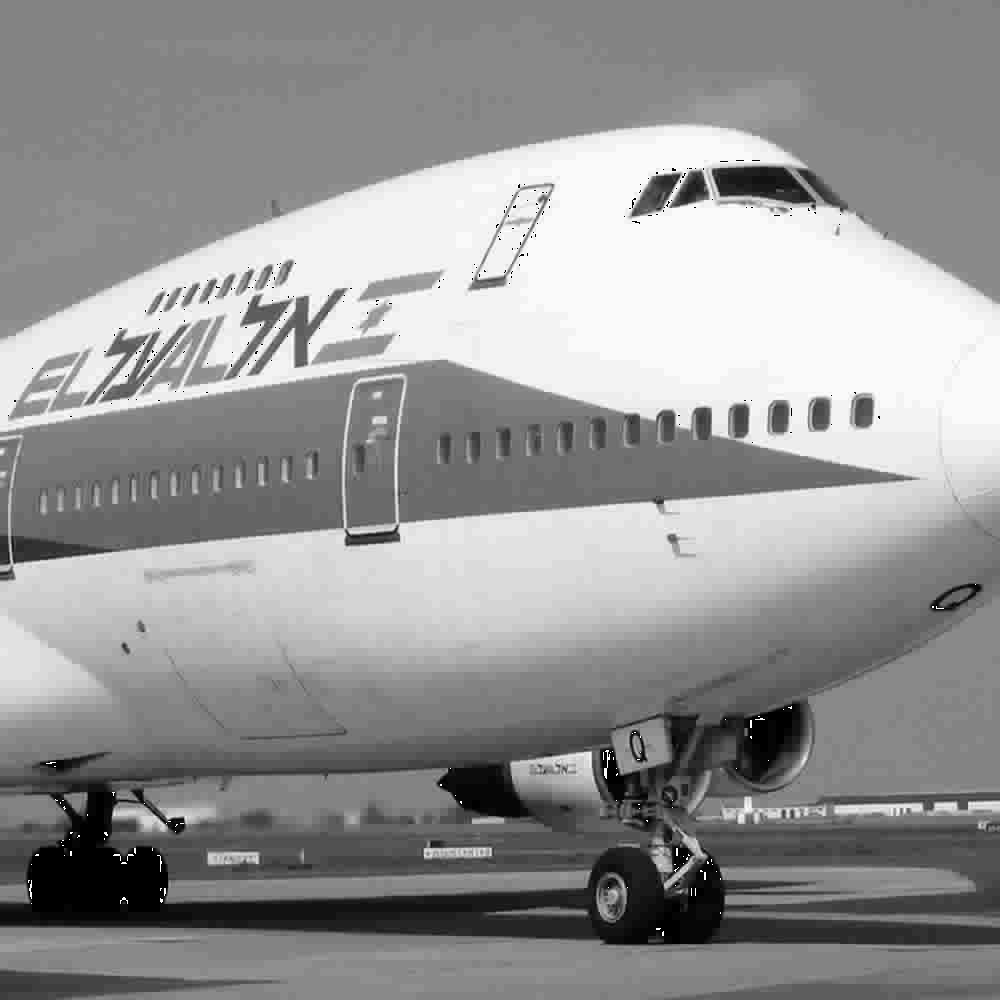
\includegraphics[width=3cm]{../imgs/output/gray_8_50_2000/img08.png} \\
\hline
img9 & 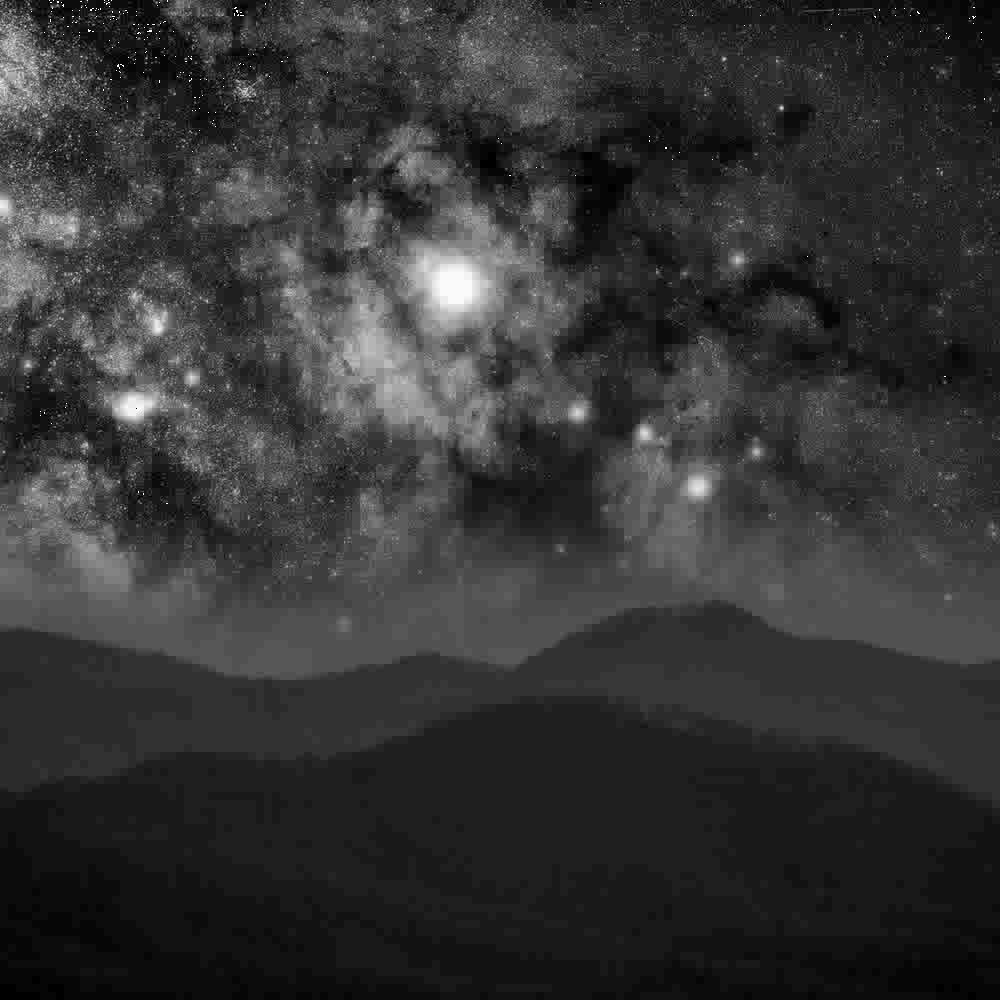
\includegraphics[width=3cm]{../imgs/output/gray_8_50_2000/img09.png} &&&& \\
\hline
\end{tabular}
\end{center}
\caption{Imágenes comprimidas con parámetros $B=8, Q=50, U=2000$}
\label{fig:imagenes_de_prueba_comprimidas_8_50_2000}
\end{figure}

\section*{Referencias}

\begin{itemize}
\item[[1]] .
\end{itemize}

\end{document}

